Bassed on the desired functionality of the platform described in the previous chapter, I was able to create a design for the user interface -- UI of the mobile application.

In the beginning of this UI design project, I first looked at what would be the platform the project should run on.
Since it is a mobile application, the range of options was slimmed down to two -- either Android or iOS,
given their prevalence on the market (Android on the first place with 70.68\% of the market share, iOS second with 28.79\% as of April 2020)~\cite{market-share-mobile-os}.
It is partially due to Android's crushing lead on iOS devices, but also because of my personal experience with the more popular OS, that I decided to design the app for Android.

One of the most important decisions to make when designing an application is the navigation in it, and from there there's only a small step to information architecture (IA) -- the \textit{science of organizing and structuring content of the [\dots] mobile applications}~\cite{information-architecture}.
The IA of an application helps the designer decide which concepts in the application are high-level and discrete enough
to be used as `umbrella terms' for navigating to other, deeper concepts, while feeling intuitive to the user.

However, when reading up on design guidelines for either of the systems, I realised that Android's instructions seem outdated.
Backed by plenty of discussions online~\cite{hamburger-discoverabillity} as well as my own user experience with the native applications, the typical hamburger menu ☰ has gone out of style.

One of the reasons is the increasing size of handheld devices.
A hamburger menu (or `navigation drawer') located in the top left corner is nearly inaccessible for the majority of users, who are right-handed and use their thumb to operate the device~\cite{thumb-zone-article}.

\begin{figure}[h!]
    \centering
    \tmpframe{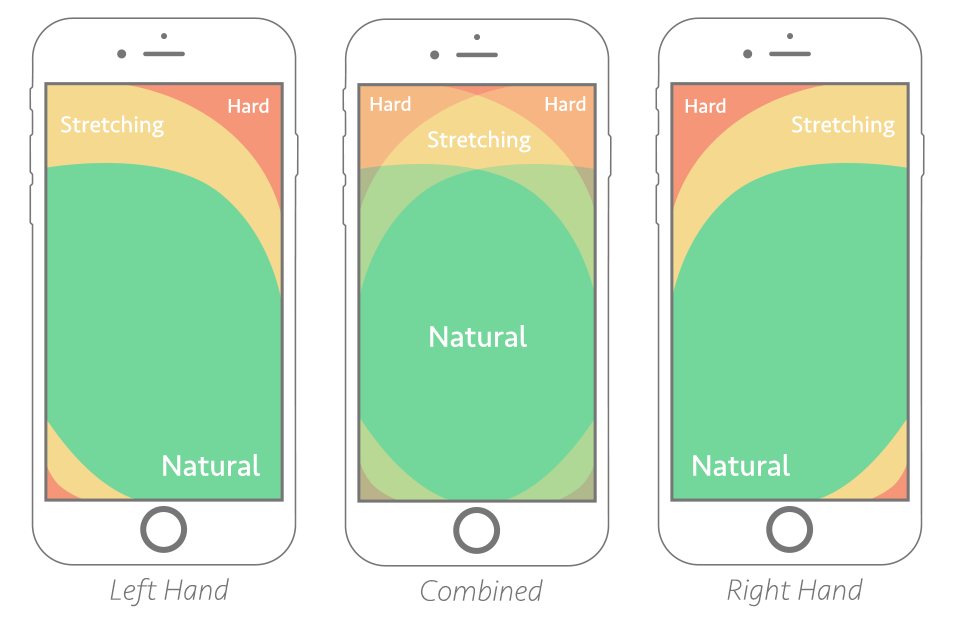
\includegraphics[width=\textwidth]{Images/thumb-zone.png}}\hfill
    \caption{Thumb-zone mapping for left- and right-handed users~\cite{thumb-zone-img}}
    \label{fig:sign-up-email}
\end{figure}

Another reason is the fact that the hamburger menu decreases discoverability of features, as they are hidden by default~\cite{hamburger-discoverabillity}.

Lastly, using the hamburger menu often tempts the designer to just put everything there, without giving too much consideration to the use of the features.

One of the most popular alternatives is the tab bar -- or `bottom navigation' in Android documentation.
This type of navigation is mainly implemented by Apple's designers, but is fast spreading to Android-powered devices.
It's a bar on the bottom of the screen containing three to five labelled icons representing \textit{tabs} where each leads to a different location in the app.
It enforces the idea that a user should always know where in the application they are, what they can do there and where they can go because it's always on the screen (except when the keyboard is being used).
Another one of its advantages is the possibility of inobtrusive notifications using icon badges -- little red circles in the top right corner of the icon, often containing a number to show the number of notifications.
Other navigation options include dropdown menus, scrollable menus, single page dot navigation, and others~\cite{hamburger-alternatives}.

When describing the screens I will refer to the user stories which the discussed UI component covers.

I chose the tab bar with five tabs: `Plans', `Routes', `Map', `Friends', and `Profile'.
However, when installing the APP, the user needs to set the APP up.

\section{Set up screens}
The welcome screen contains all the options for signing up, with a button to switch to the sign-in screen if the user already has an account (US~\ref{US:user-log-in}).
Signing up with e-mail creates a new account for the user based on their e-mail~(fig.\ref{fig:sign-up-email}), while using a social network account takes the user to a sign-in screen of the specific social network.
Similarly, the user can sign in to their existing account~(fig.\ref{fig:sign-in-email}).

\begin{figure}[h!]
    \centering
    \tmpframe{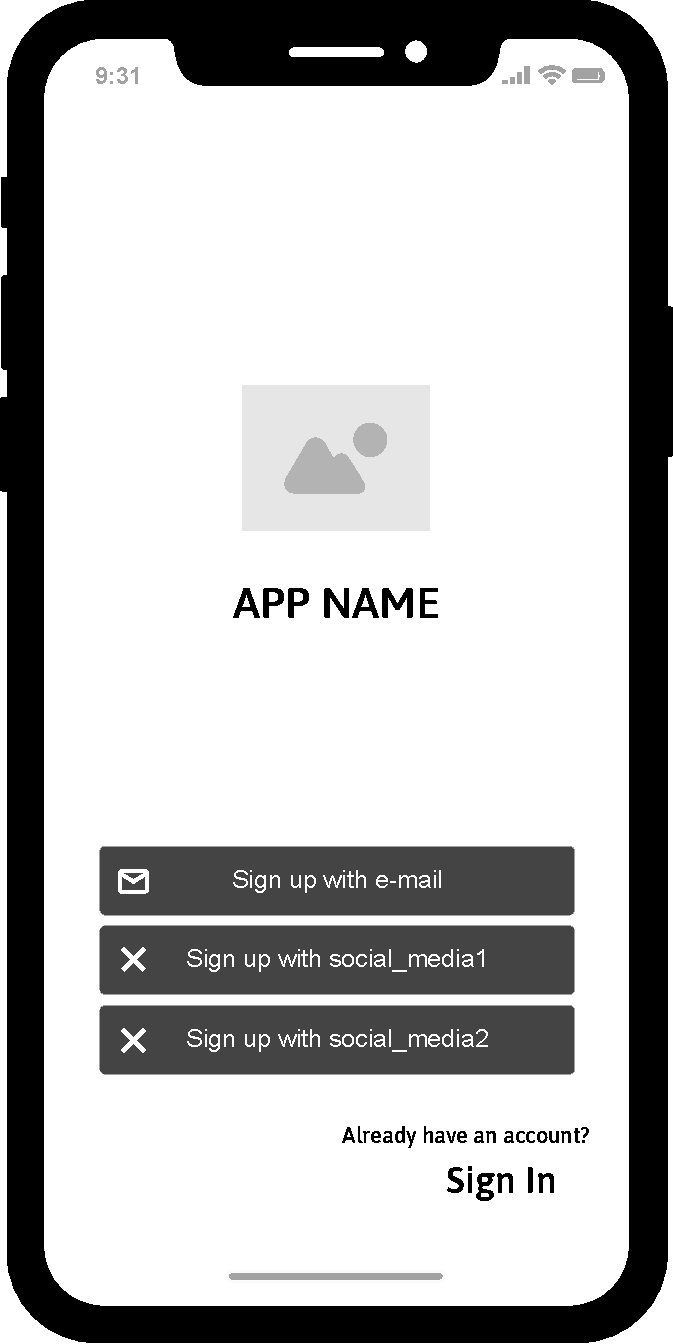
\includegraphics[width=0.4\textwidth]{Images/appScreens/signUp1.pdf}}\hfill
    \tmpframe{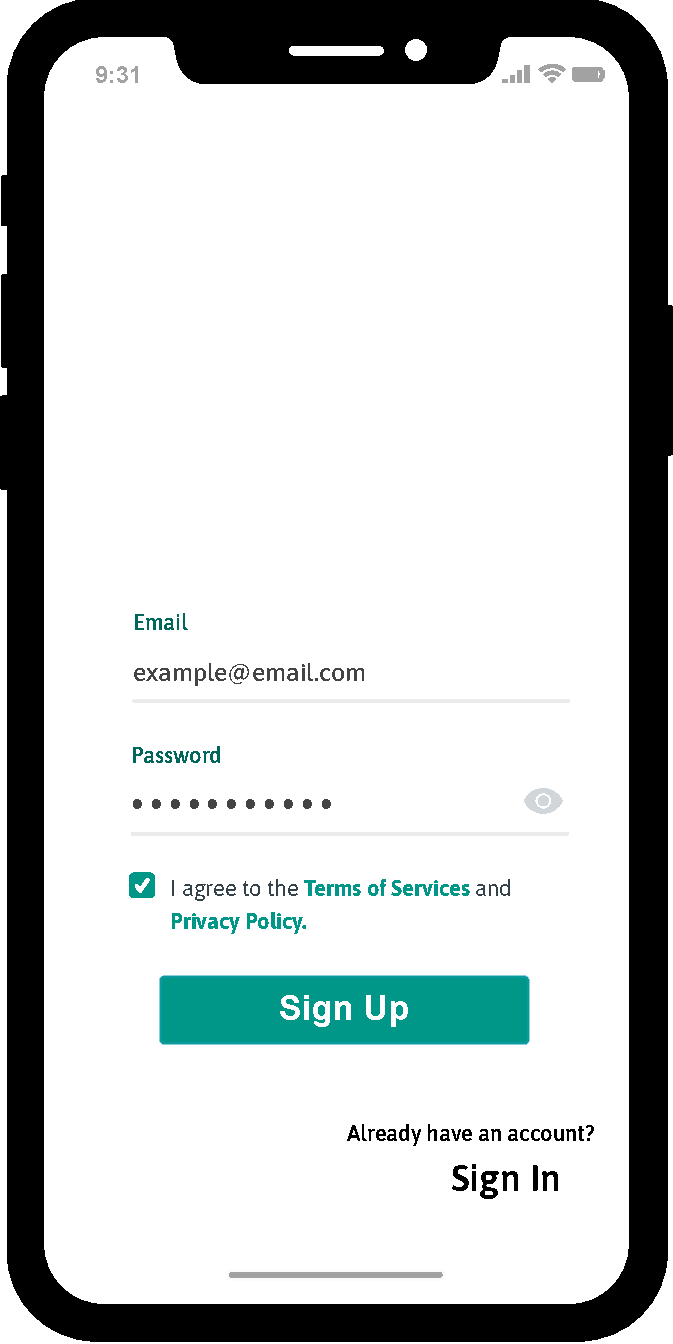
\includegraphics[width=0.4\textwidth]{Images/appScreens/signUp2.pdf}}
    \caption{Welcome screen with sign-up options and e-mail sign-up screen}
    \label{fig:sign-up-email}
\end{figure}

\begin{figure}[h!]
    \centering
    \tmpframe{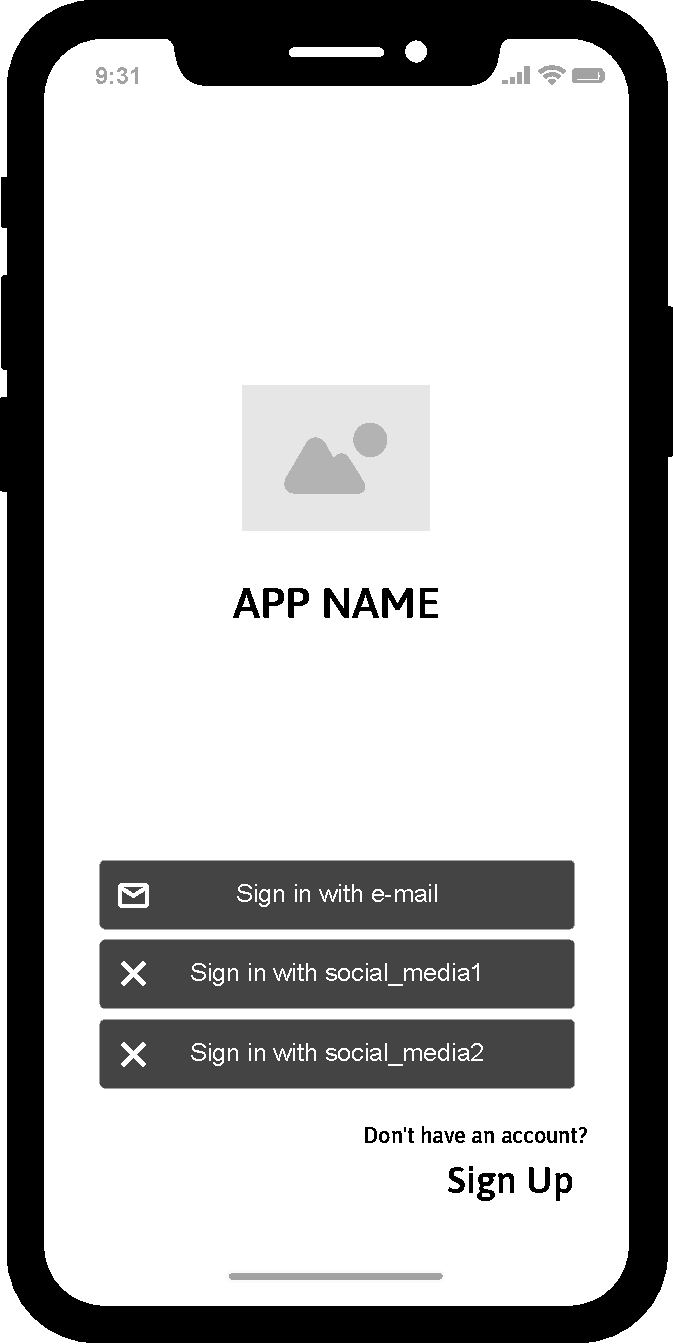
\includegraphics[width=0.4\textwidth]{Images/appScreens/signIn1.pdf}}\hfill
    \tmpframe{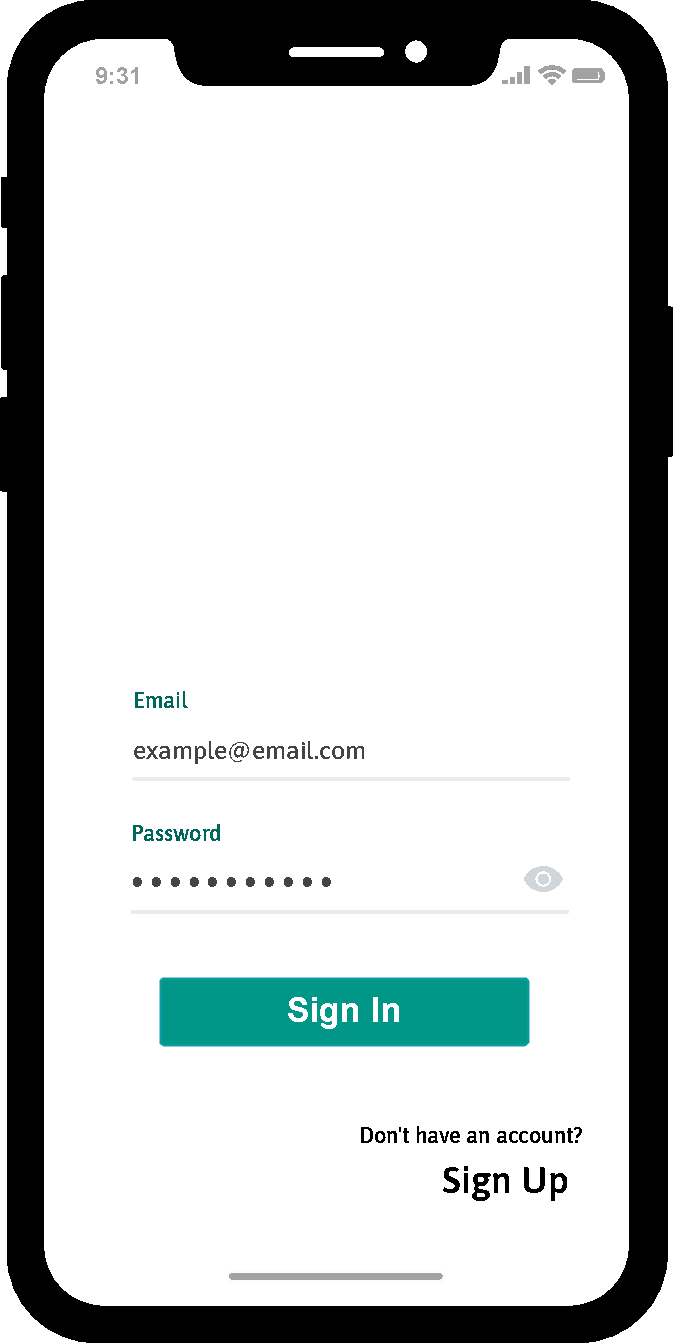
\includegraphics[width=0.4\textwidth]{Images/appScreens/signIn2.pdf}}
    \caption{Welcome screen with sign-in options and e-mail sign-in screen}
    \label{fig:sign-in-email}
\end{figure}

After signing up and creating a new account, there is a sequence of screens asking for the user's personal data, such as height, weight, biological sex, birth date, and whether they know about a condition that means their heart rate should be limited, and if so, how much (on a scale of 1 to 5) (US~\ref{US:manual-advanced}, \ref{US:manual-basic}).
Another screen asks the user to pair a watch with the APP, showing a list of Bluetooth devices paired with the phone (US~\ref{US:HRM-device-management}).
The last one asks the user to take a fitness test, so that their fitness can be assessed (epic~\ref{epic:fit}).
This step can be skipped, but there's a warning about the inaccuracy of methods based on readily available data compared to taking a fitness test.
At the same time, the user is assured that the test can be taken later.

If the user decides to take the test, they are rerouted to the screen with fitness tests (without the bottom navigation bar).
Again, it is possible to quit this screen.

\section{Profile tab}
After setup, the APP opens on the `Profile' tab, displaying all entered and calculated information on cards, as well as the option to log out, and the currently active device~(fig.\ref{fig:profile1}; US~\ref{US:user-manage-info}, \ref{US:user-log-in}, \ref{US:HRM-device-activate}).

\begin{figure}[h!]
    \centering
    \tmpframe{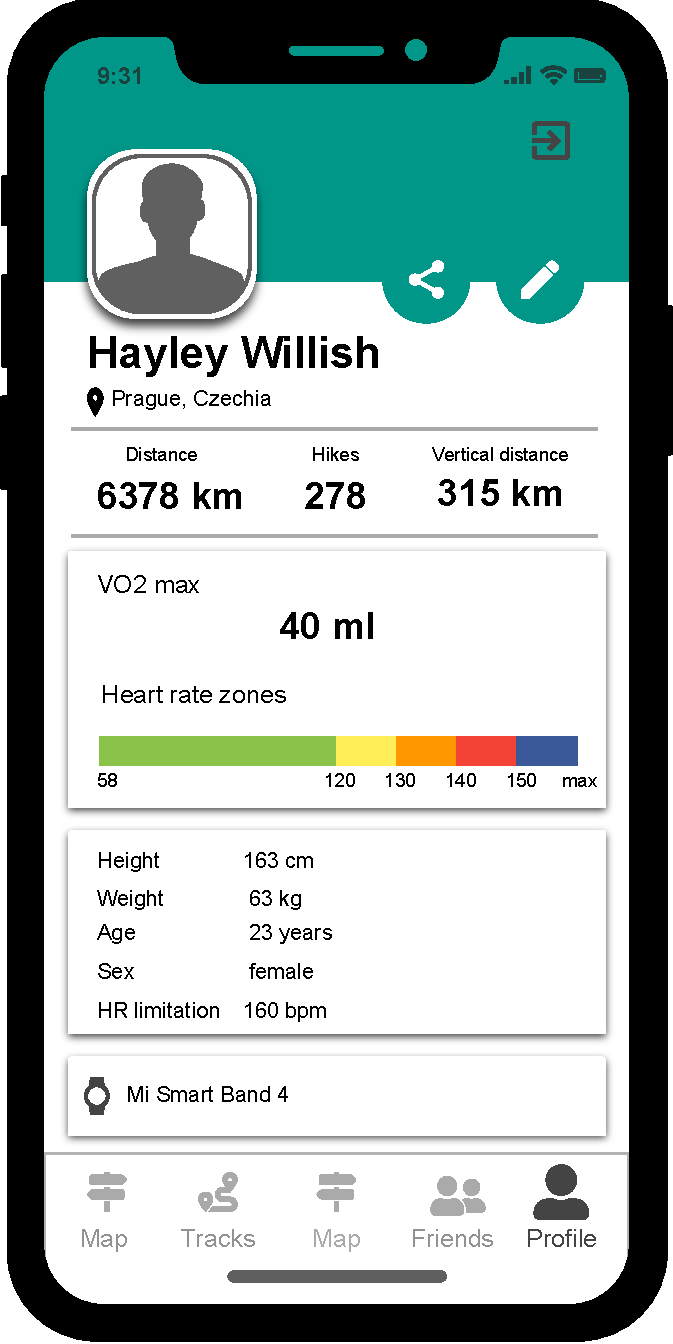
\includegraphics[width=0.4\textwidth]{Images/appScreens/profile1.pdf}}\hfill
    \caption{The Profile screen}
    \label{fig:profile1}
\end{figure}

The card with fitness opens to show the user's fitness data -- VO2 max, heart rate zones, and minimum and maximum heart rate.
The heart rate zones are color-coded; these colors occur in the whole application to signify difficulty.
There's an icon to get more information about the metrics (excerpts from the Fitness Assessment chapter), and the option to take a fitness test~(fig.\ref{fig:fitnessInfo}).
The pictures are placeholders for charts of development of the metric over time.

\begin{figure}[h!]
    \centering
    \tmpframe{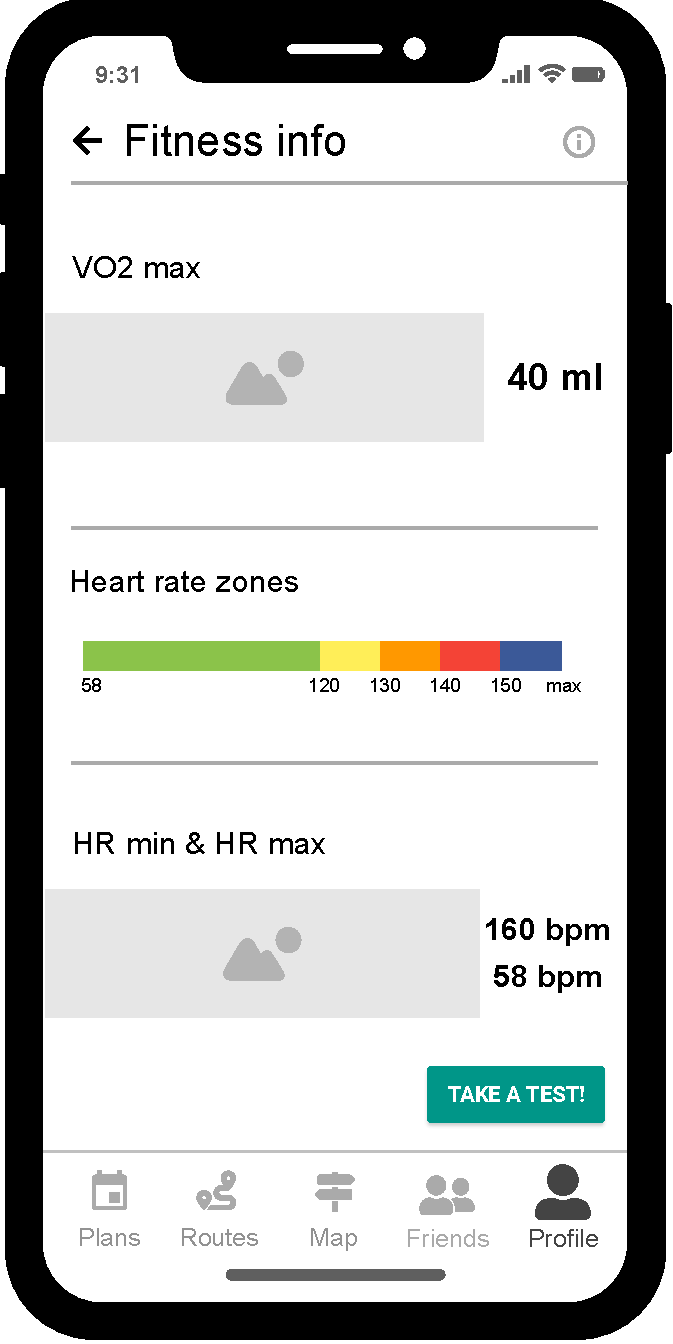
\includegraphics[width=0.4\textwidth]{Images/appScreens/profile-fitnessInfo.pdf}}\hfill
    \caption{Fitness information}
    \label{fig:fitnessInfo}
\end{figure}

On the `Fitness tests' screen, the user can choose between multiple tests, each of which has a tag saying what it tests(fig.\ref{fig:fitnessTests}; epic~\ref{epic:fit}).
As an example, the `6 Minute Walking Test' screen has directions on what the user should do, and after the test, there is a screen with results~(fig.\ref{fig:6mwt}).
Again, the pictures will contain the charts of the metric's values over the course of the test.

\begin{figure}[h!]
    \centering
    \tmpframe{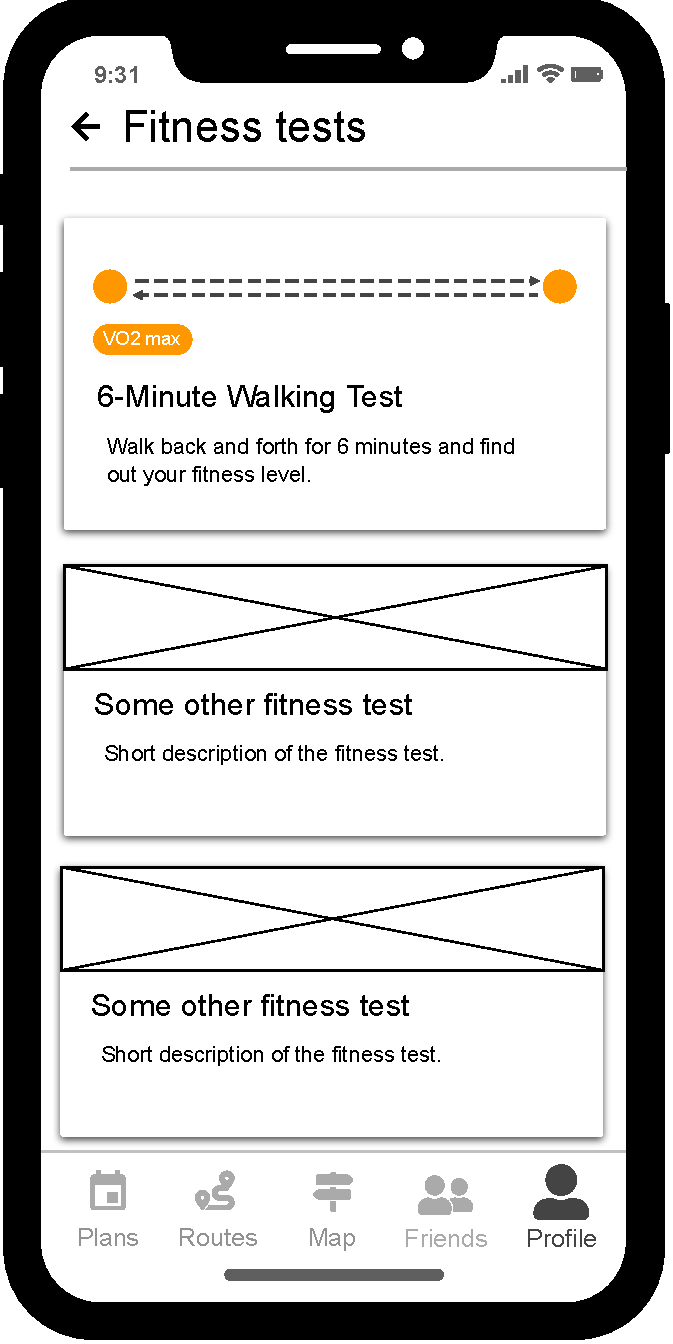
\includegraphics[width=0.4\textwidth]{Images/appScreens/profile-fitnessTests.pdf}}\hfill
    \caption{Fitness tests}
    \label{fig:fitnessTests}
\end{figure}

\begin{figure}[h!]
    \centering
    \tmpframe{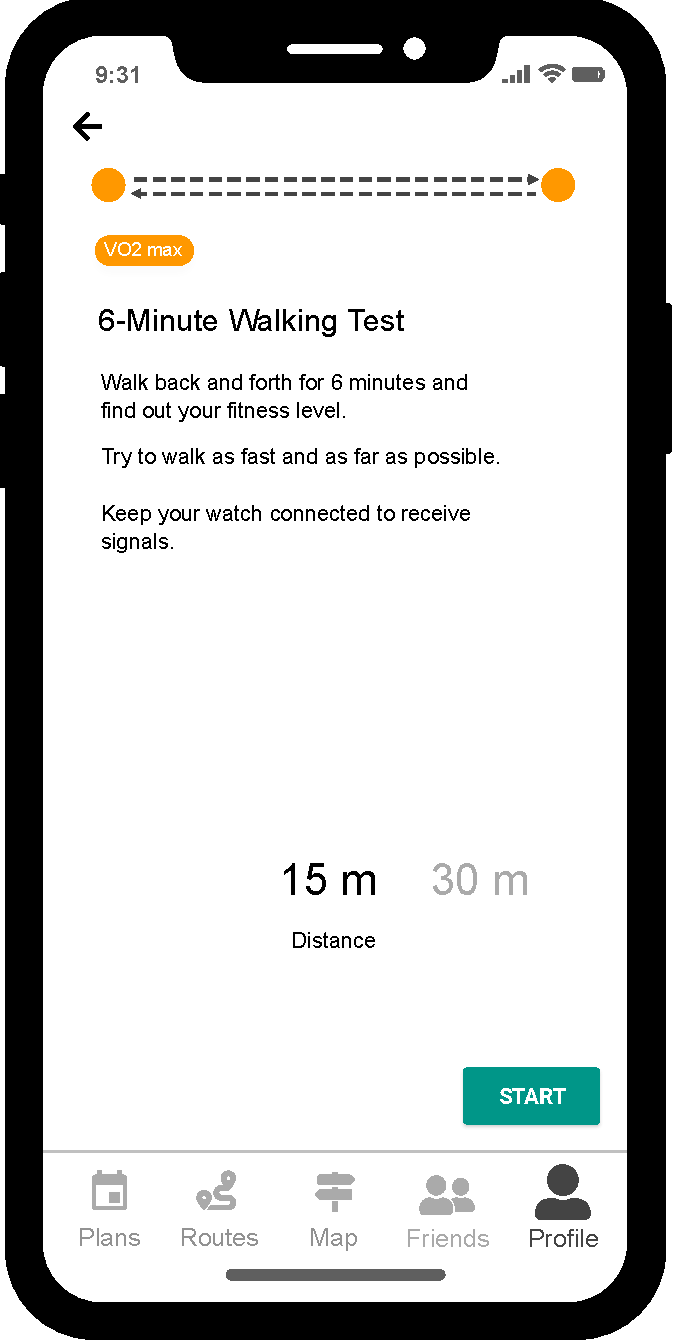
\includegraphics[width=0.4\textwidth]{Images/appScreens/profile-fitness-6mwt.pdf}}\hfill
    \tmpframe{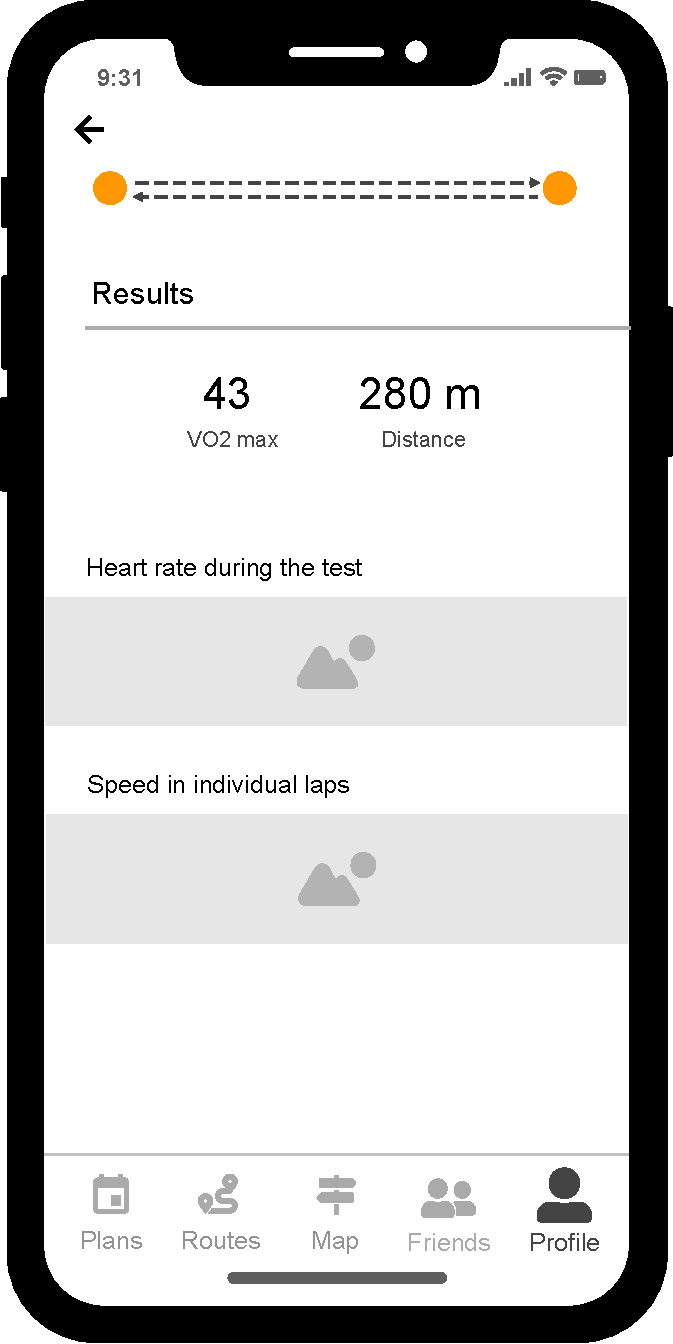
\includegraphics[width=0.4\textwidth]{Images/appScreens/profile-fitness-6mwt-results.pdf}}
    \caption{6 Minute Walking Test}
    \label{fig:6mwt}
\end{figure}

When we come back to the `Profile' screen (fig.\ref{fig:profile1}), we can also manually edit all the information the user has provided.
The profile picture, basic data like height etc., as well as the fitness information (US~\ref{epic:manual}, \ref{US:user-manage-pic}).

Another option from here is to see the devices by expanding the card with the active device.
The `Devices' screen~(fig.\ref{fig:devices}) contains the active device which can be deactivated (US~\ref{US:HRM-device-activate}, \ref{US:HRM-device-management}), as well as other paired devices, which can be either activated or unpaired.
The user can also pair a new device with the app (opening a list of devices paired with the phone).
Tapping the `Activate' button will deactivate the currently active device.

\begin{figure}[h!]
    \centering
    \tmpframe{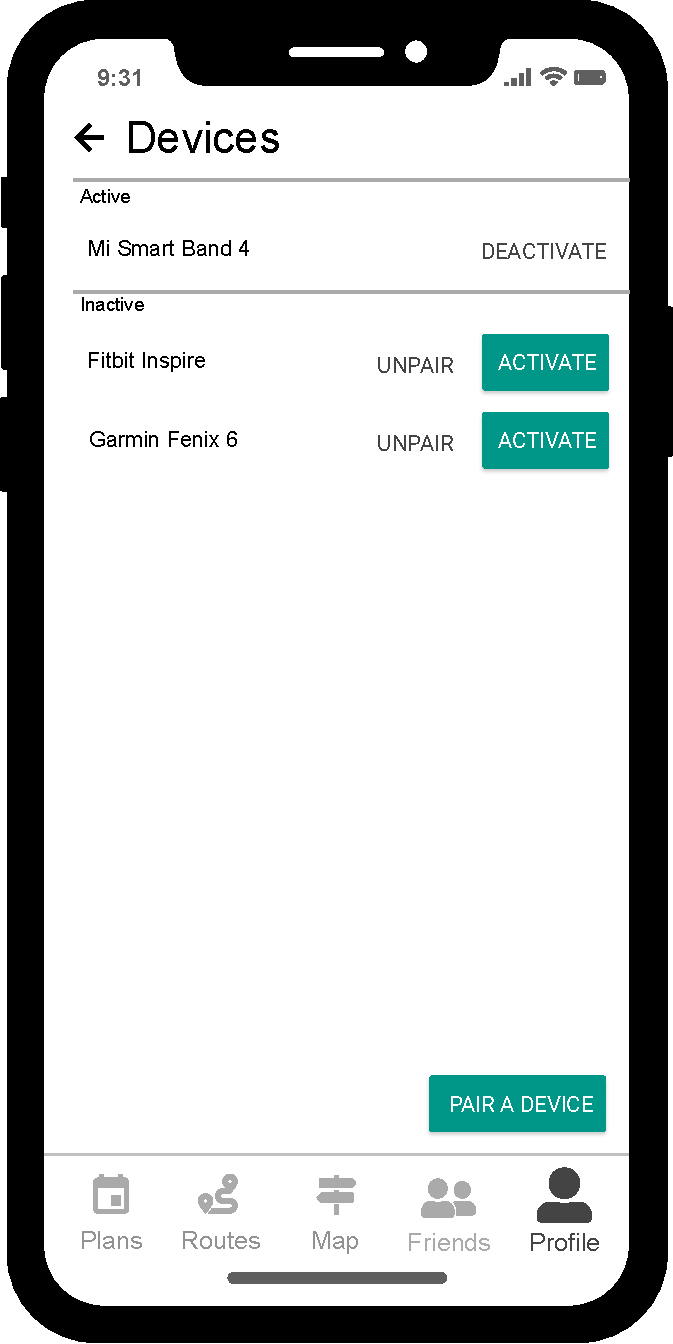
\includegraphics[width=0.4\textwidth]{Images/appScreens/profile-devices.pdf}}\hfill
    \caption{Devices}
    \label{fig:devices}
\end{figure}

\section{Map tab}
The default tab on which the application opens is the `Map' tab~(fig.\ref{fig:map}).
This is where the user can look at the integrated map (US~\ref{US:map-integrate}), as well as search for specific places~(fig.\ref{fig:map-searchPlace}) and add them as waypoints to the planned route (US~\ref{US:map-plan}).
The waypoint will be added to the route as the `next' waypoint.

\begin{figure}[h!]
    \centering
    \tmpframe{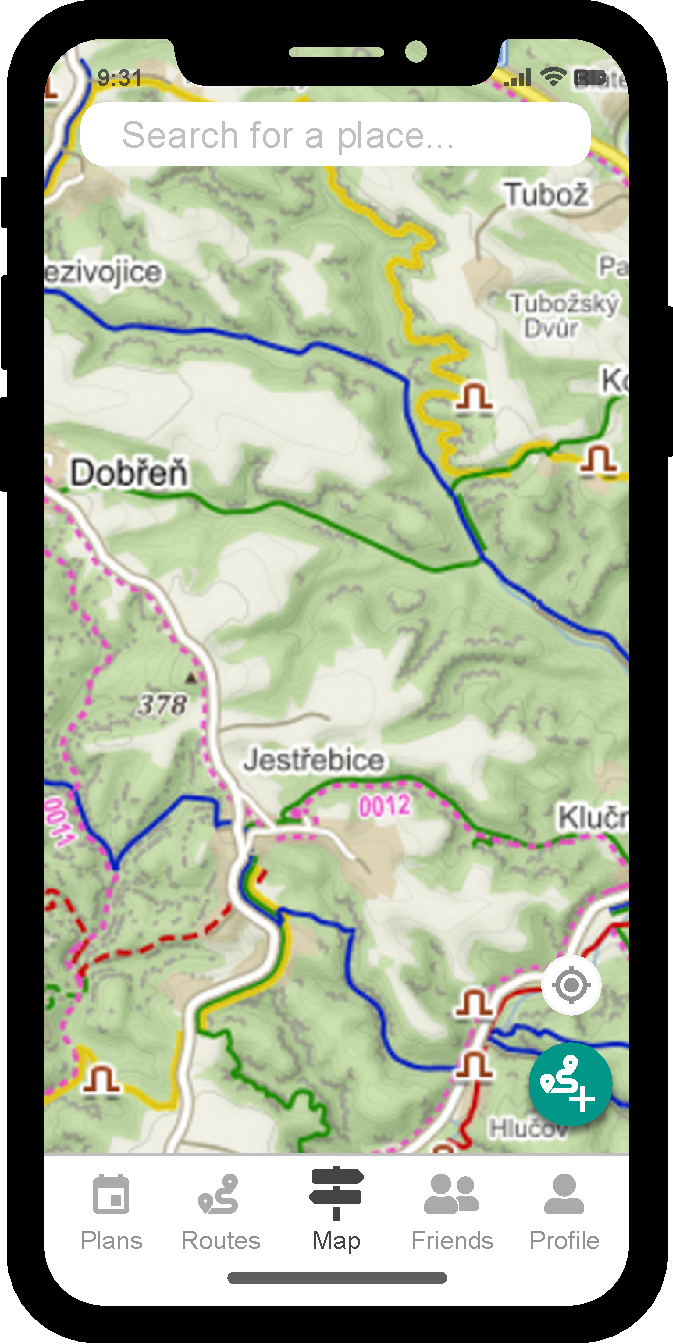
\includegraphics[width=0.4\textwidth]{Images/appScreens/maps1.pdf}}\hfill
    \caption{Map screen}
    \label{fig:map}
\end{figure}

\begin{figure}[h!]
    \centering
    \tmpframe{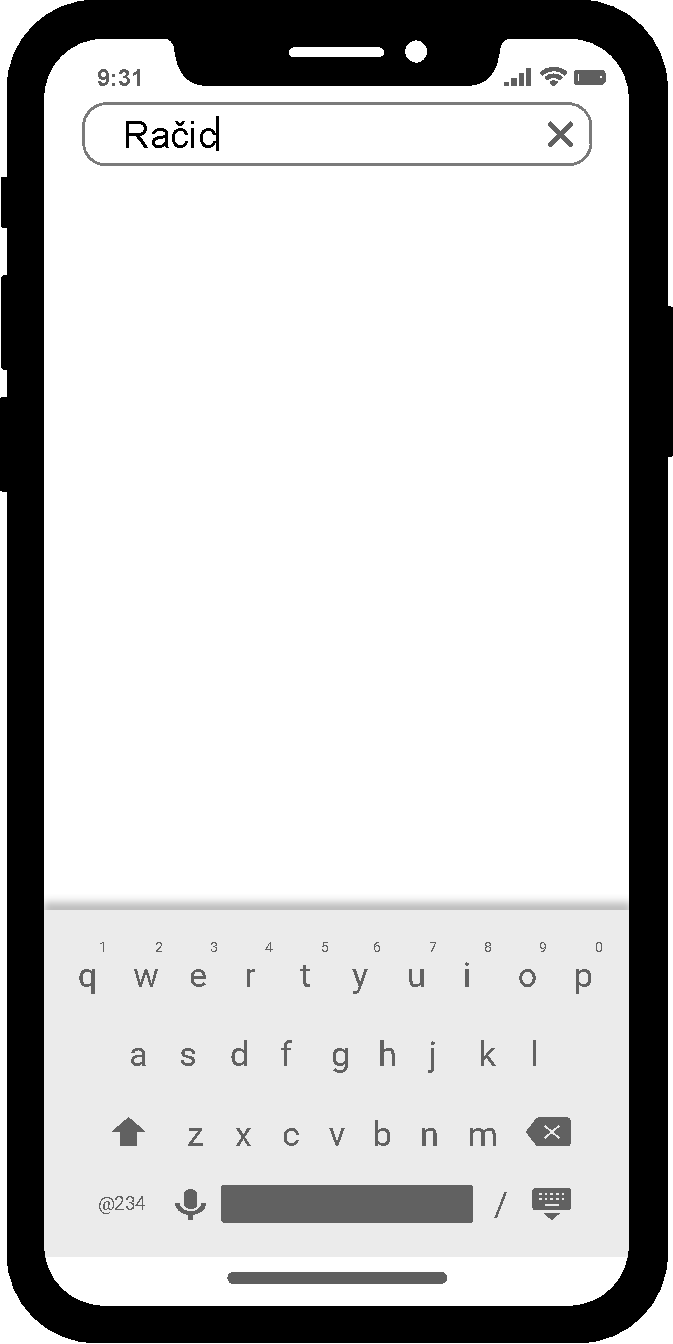
\includegraphics[width=0.3\textwidth]{Images/appScreens/map-search1.pdf}}\hfill
    \tmpframe{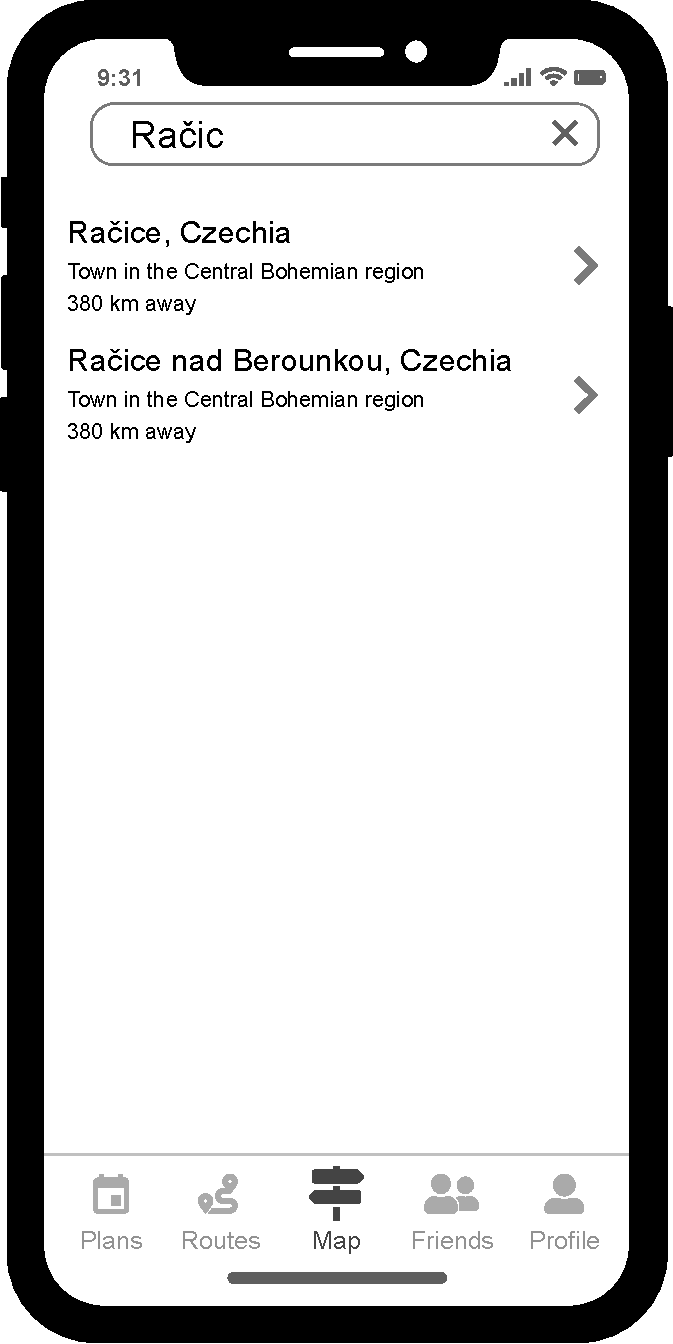
\includegraphics[width=0.3\textwidth]{Images/appScreens/map-search2.pdf}}\hfill
    \tmpframe{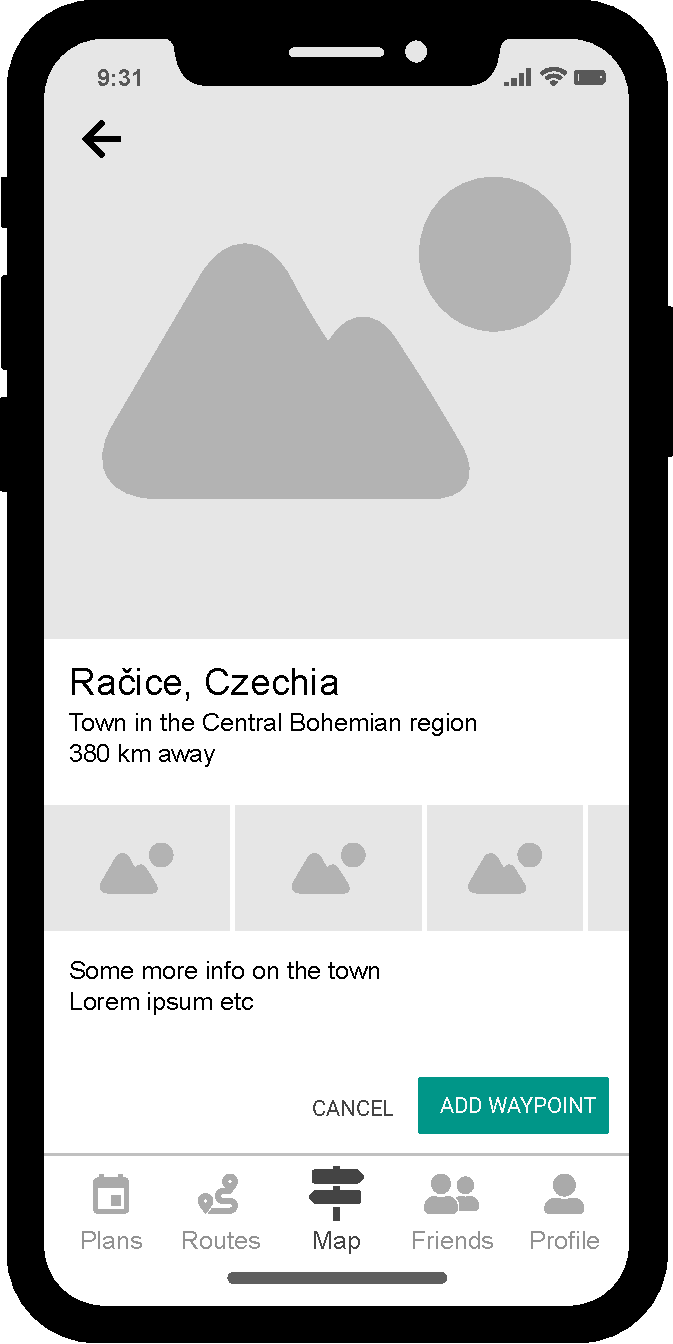
\includegraphics[width=0.3\textwidth]{Images/appScreens/map-search3.pdf}}\hfill
    \caption{Search for a place}
    \label{fig:map-searchPlace}
\end{figure}

Planning a new route can also be started with the floating button on the bottom right of the screen~(fig.\ref{fig:map}).

The planning process consists of three steps:
\begin{enumerate}
    \item waypoints,
    \item pick a route, and
    \item plan a hike.
\end{enumerate}

In the `Waypoints' step~fig.\ref{fig:plan-waypoints}), the user picks where they want to start their route, the destination, and all the points through which they want to pass.
Each of the points can be picked directly from the map with a long press, or by searching for a place~(fig.\ref{fig:map-searchPlace}).
The current location can also be used as a starting point.
The intermediate points can be added using the plus button, and all the waypoints can be rearranged by drag'n'dropping each line by the menu icon on the left.
The user can also remove individual waypoints using the X icon on the right: when removing the starting or destination point, only the text is removed, since every route needs two points.

Another option is to choose a return trip, where the platform should offer routes that start in the starting point, go through the destination, and either give a different route to go back if possible, or has the user retrace their steps.

\begin{figure}[h!]
    \centering
    \tmpframe{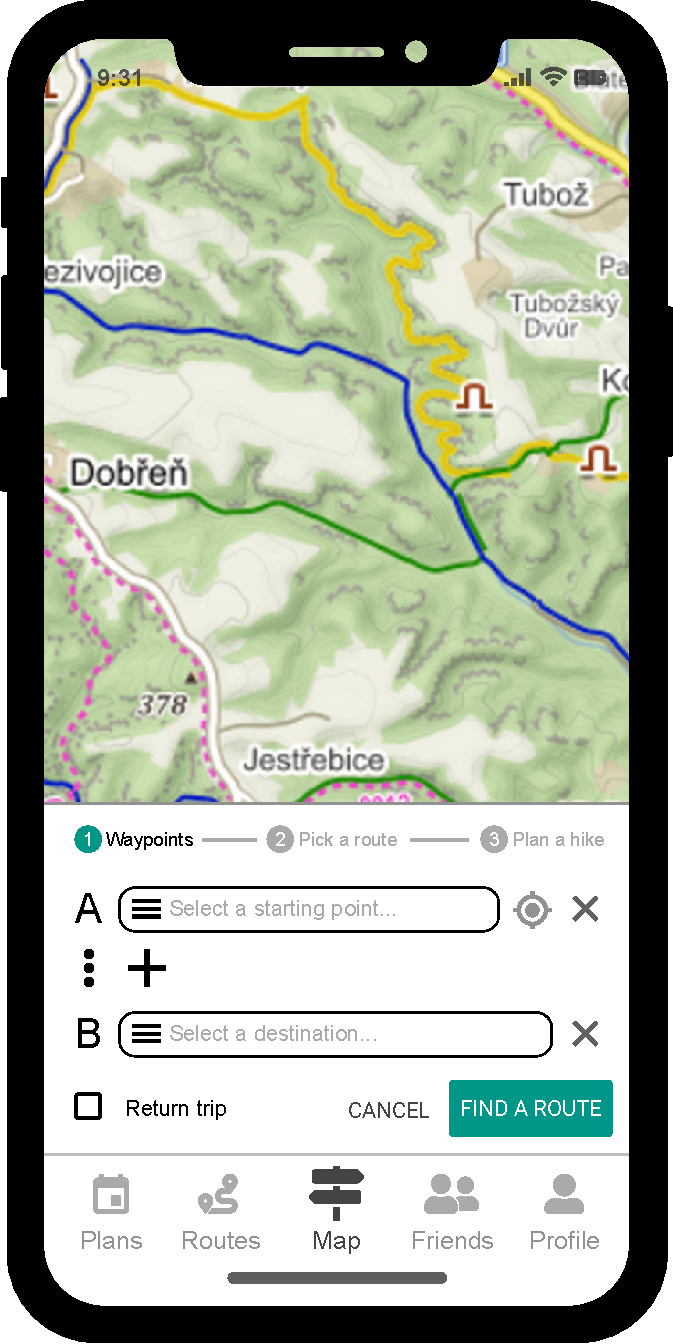
\includegraphics[width=0.4\textwidth]{Images/appScreens/map-plan1.pdf}}\hfill
    \tmpframe{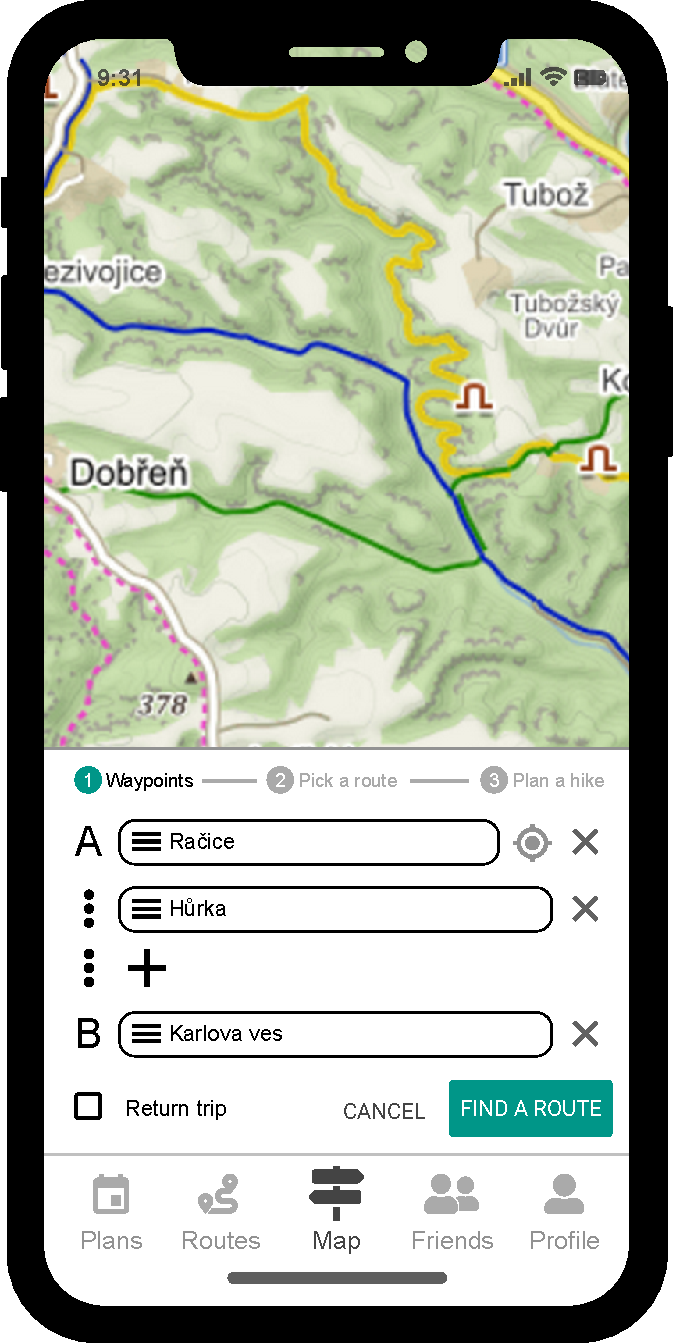
\includegraphics[width=0.4\textwidth]{Images/appScreens/map-plan2.pdf}}\hfill
    \caption{Planning a route with waypoints}
    \label{fig:plan-waypoints}
\end{figure}

When the user is satisfied with the waypoints, they tap the `Find a route' button.
In this step the planning UI pulls up higher, covering a larger part of the map, while the visible part of the map contains all the route options on an appropriately zoomed-in map.
The options are colour-coded based on their difficulty.
The chosen option is highlighted, while the others are visible but translucent.
The options can be switched between by tapping on the map.

The middle of the planning UI now contains the details of the chosen route -- the time it will get the user to hike it if they go alone, its elevation, length, prevalent surface type, and a difficulty chart (US~\ref{US:map-planned-details}).

The bottom part of the planning UI has information on individual segments of the route.
The picture is a placeholder for the route's elevation profile, which has two interactive sliders to pick the segment whose details the user wants to know.
These details include its elevation, surface, and a difficulty chart.

The route can be saved and unsaved by tapping the bookmark icon, and shared via link by tapping the share icon.

If the user wants to just start the hike without planning for a different day or inviting friends, they can press the `GO' button and the APP navigates them,
or they can continue to the next step: Plan a hike.

\begin{figure}[h!]
    \centering
    \tmpframe{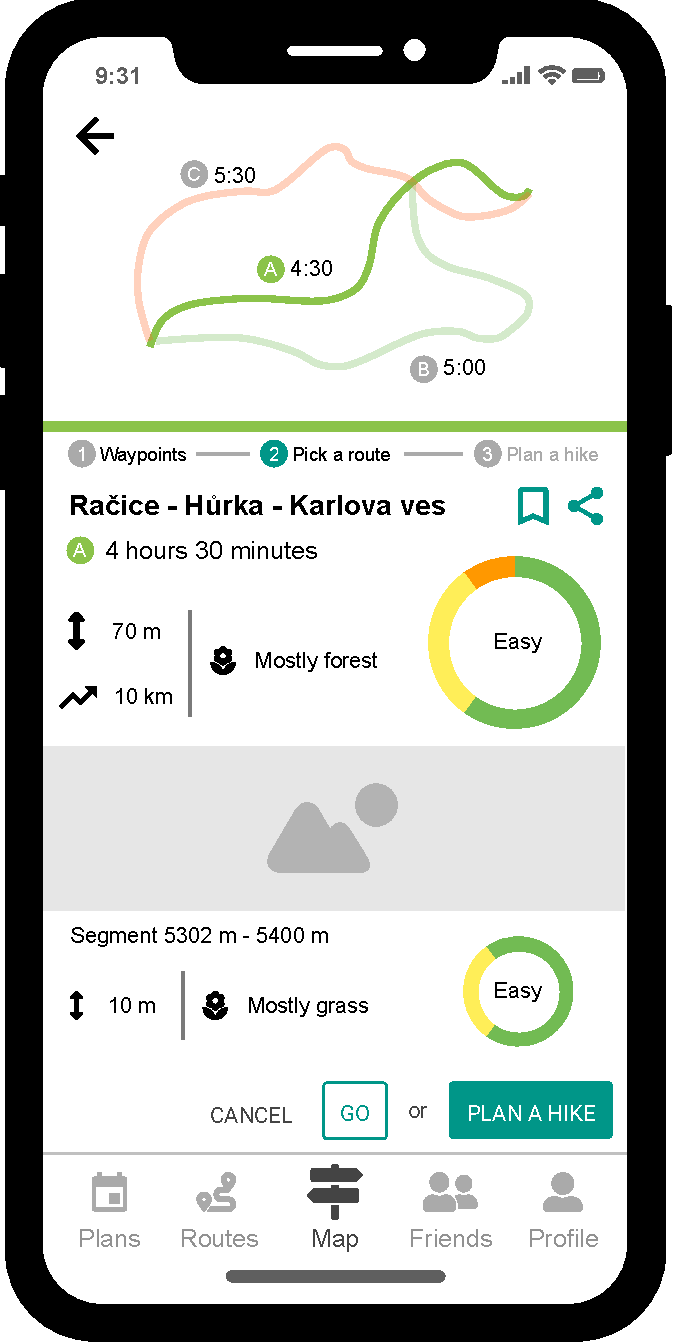
\includegraphics[width=0.4\textwidth]{Images/appScreens/map-plan3.pdf}}\hfill
    \tmpframe{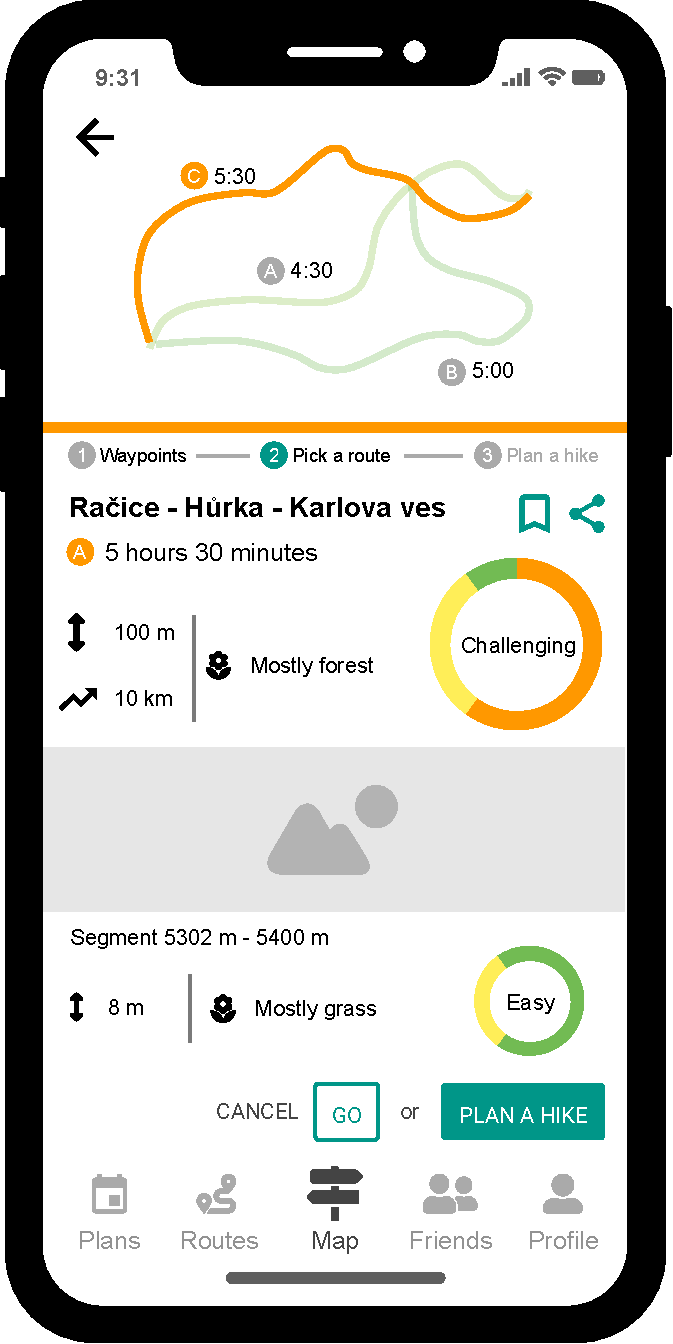
\includegraphics[width=0.4\textwidth]{Images/appScreens/map-plan4.pdf}}\hfill
    \caption{Picking a route based on its details.}
    \label{fig:plan-pick-route}
\end{figure}

Planning a hike means choosing the date with a date picker (US~\ref{US:map-hike-change}), and the people to join the user~(fig.\ref{fig:plan-plan-hike}; US~\ref{US:friends-invite}).
These can be searched for among the user's friends, using the `invite people' button~(fig.\ref{fig:plan-invite-friends}).
While searching for friends, their avatars are added to the summary on the bottom and the counter is incremented.

\begin{figure}[h!]
    \centering
    \tmpframe{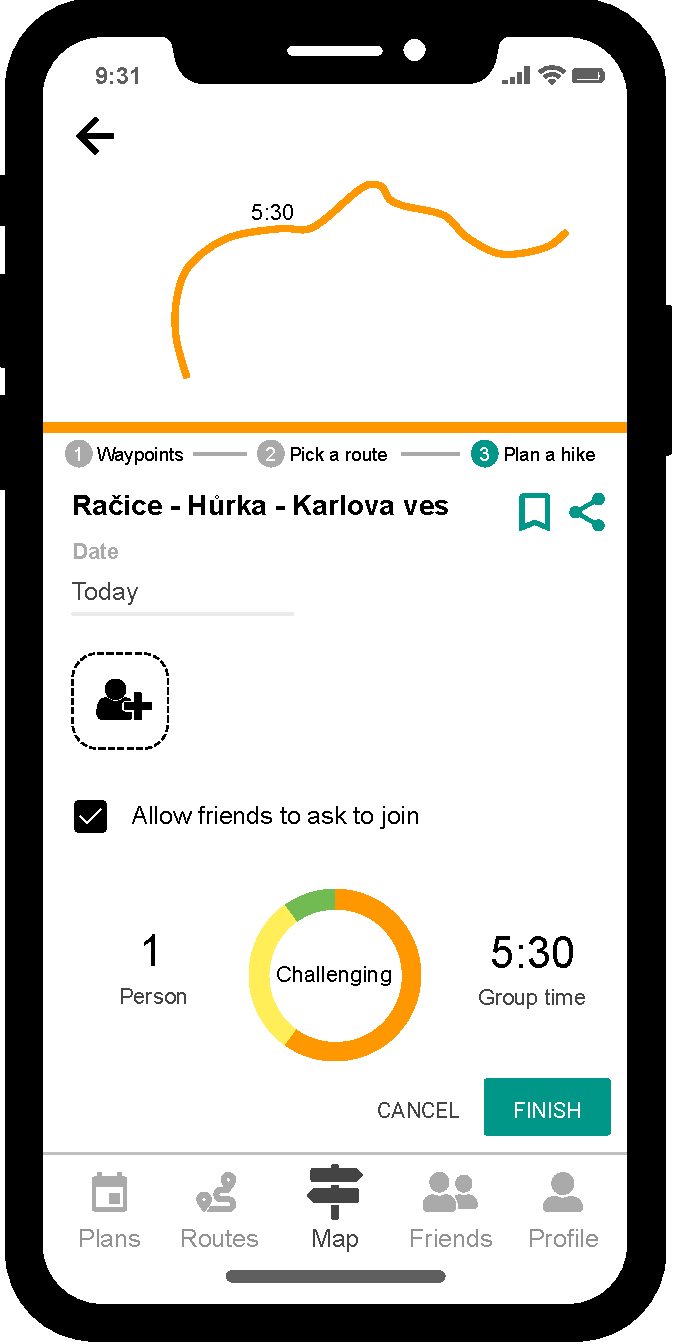
\includegraphics[width=0.4\textwidth]{Images/appScreens/map-plan5.pdf}}\hfill
    \caption{The initial state of a planned hike.}
    \label{fig:plan-plan-hike}
\end{figure}

\begin{figure}[h!]
    \centering
    \tmpframe{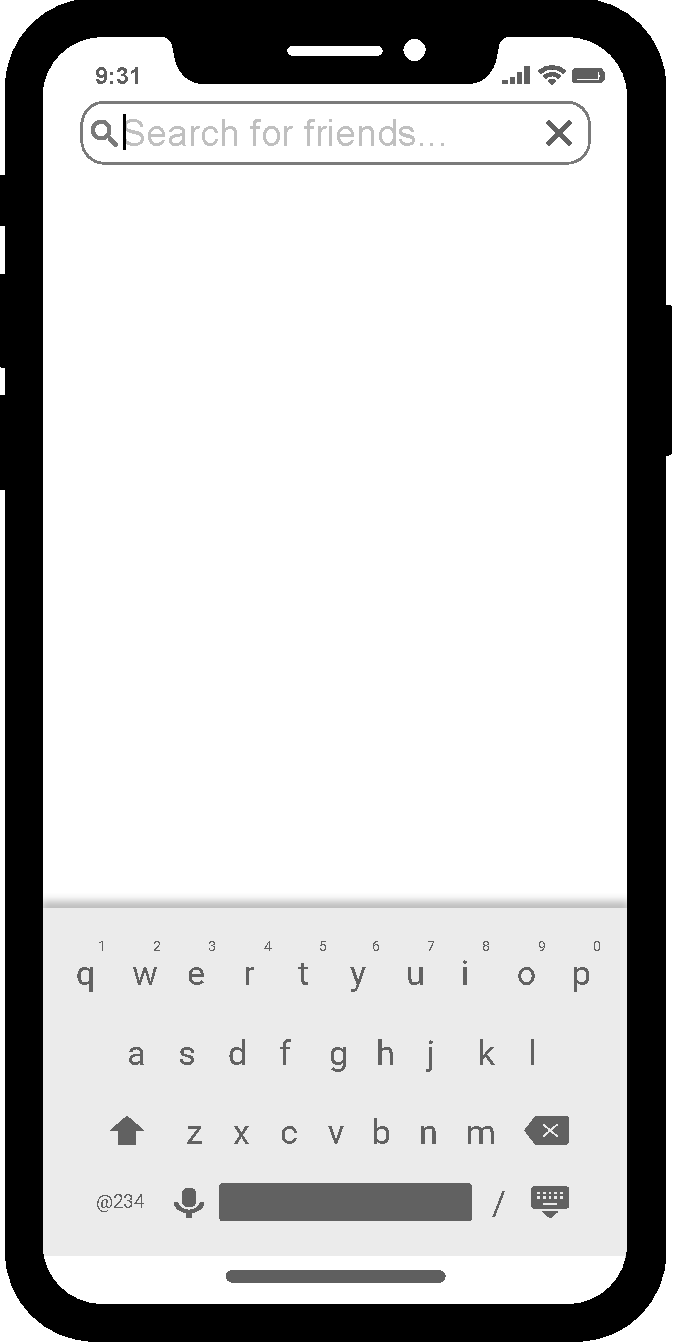
\includegraphics[width=0.4\textwidth]{Images/appScreens/map-plan6-friends.pdf}}\hfill
    \tmpframe{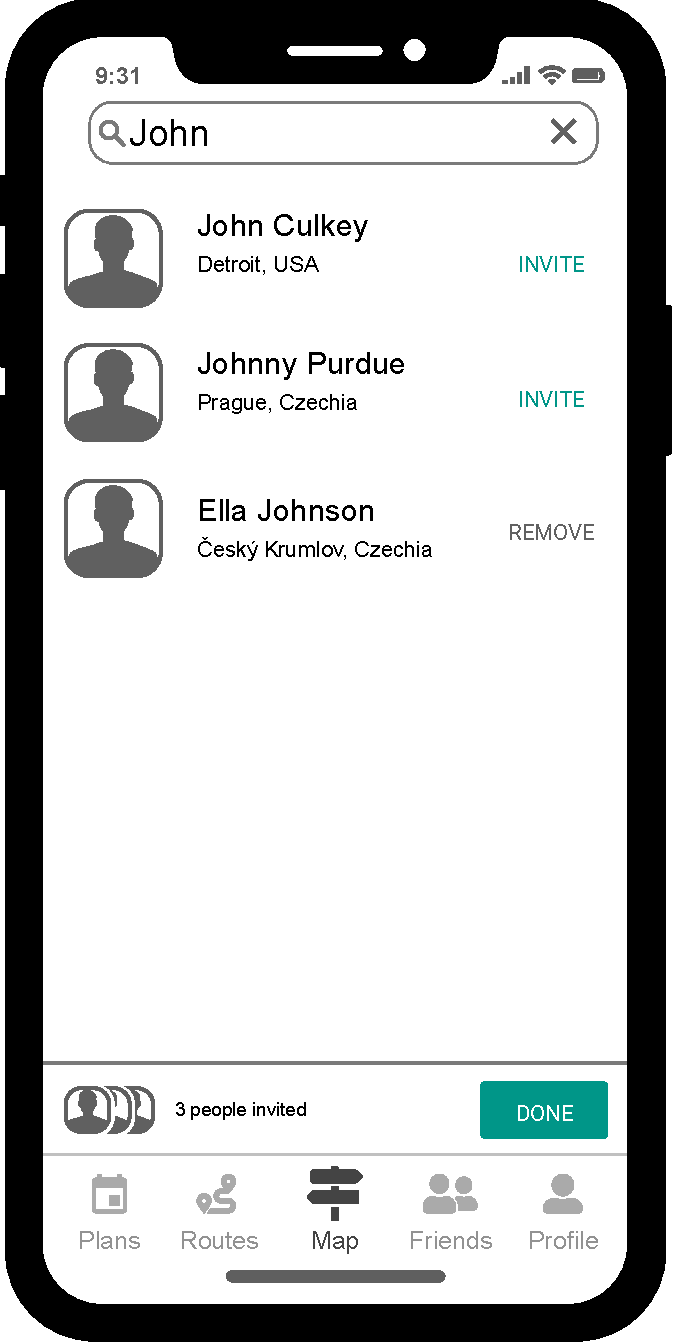
\includegraphics[width=0.4\textwidth]{Images/appScreens/map-plan7-friends.pdf}}\hfill
    \caption{Searching for friends to invite to a hike. A summary of already chosen people is on the bottom.}
    \label{fig:plan-invite-friends}
\end{figure}

Once the friends are chosen, the user can see a summary of the hike, with the difficulty chart adjusted to the group's common fitness (fig.\ref{fig:plan-end}; US~\ref{US:friends-fitness}), the number of people who are coming or invited, and how long it is going to take them.

This screen also contains a checkbox to allow friends join the hike -- whether the hike should be marked as joinable when it is shared to the friends' feed of `All plans'~(fig.\ref{fig:plan-all-plans}).

Once the planning is finished, we return to the basic `Map' screen, with a snack bar notification telling the user where they can find the planned hike and how many people were invited~(fig.\ref{fig:plan-end}).

The whole planning can be stopped at any point with the `Cancel' button, which will trigger a confirmation dialogue, as the user is about to delete all their progress, and after confirming, we return to the `Map' tab.

\begin{figure}[h!]
    \centering
    \tmpframe{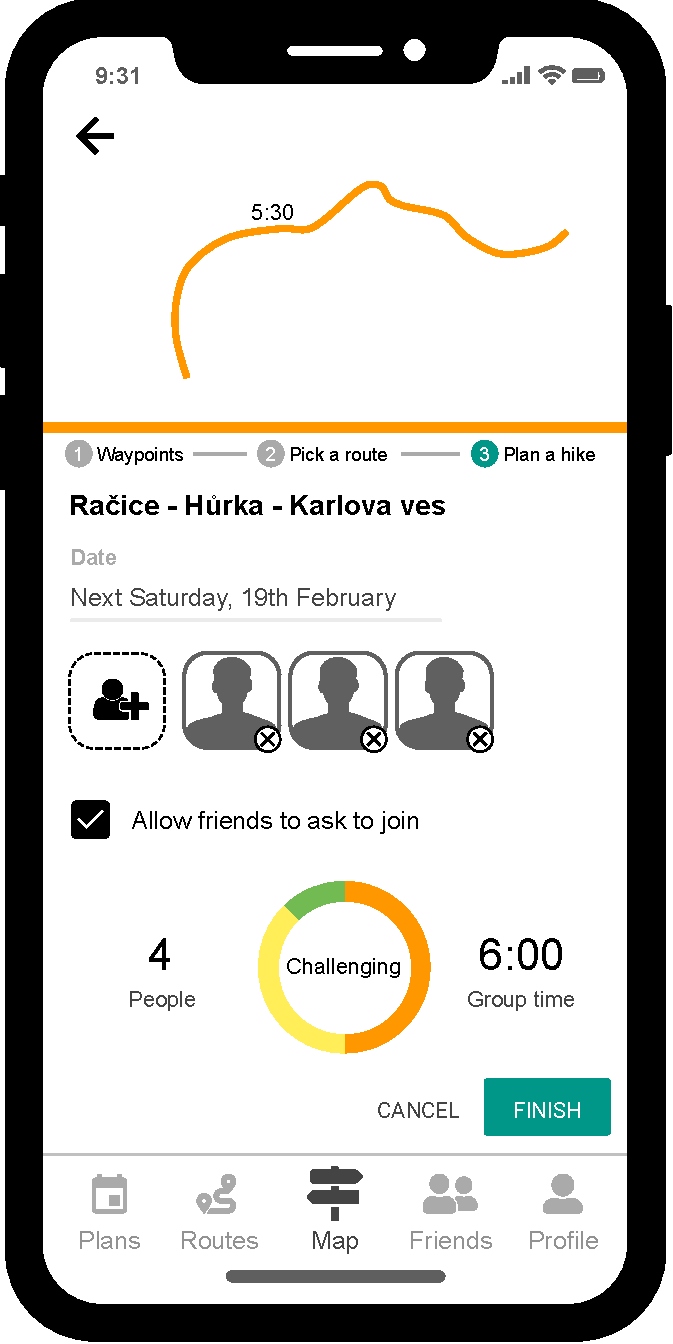
\includegraphics[width=0.4\textwidth]{Images/appScreens/map-plan8.pdf}}\hfill
    \tmpframe{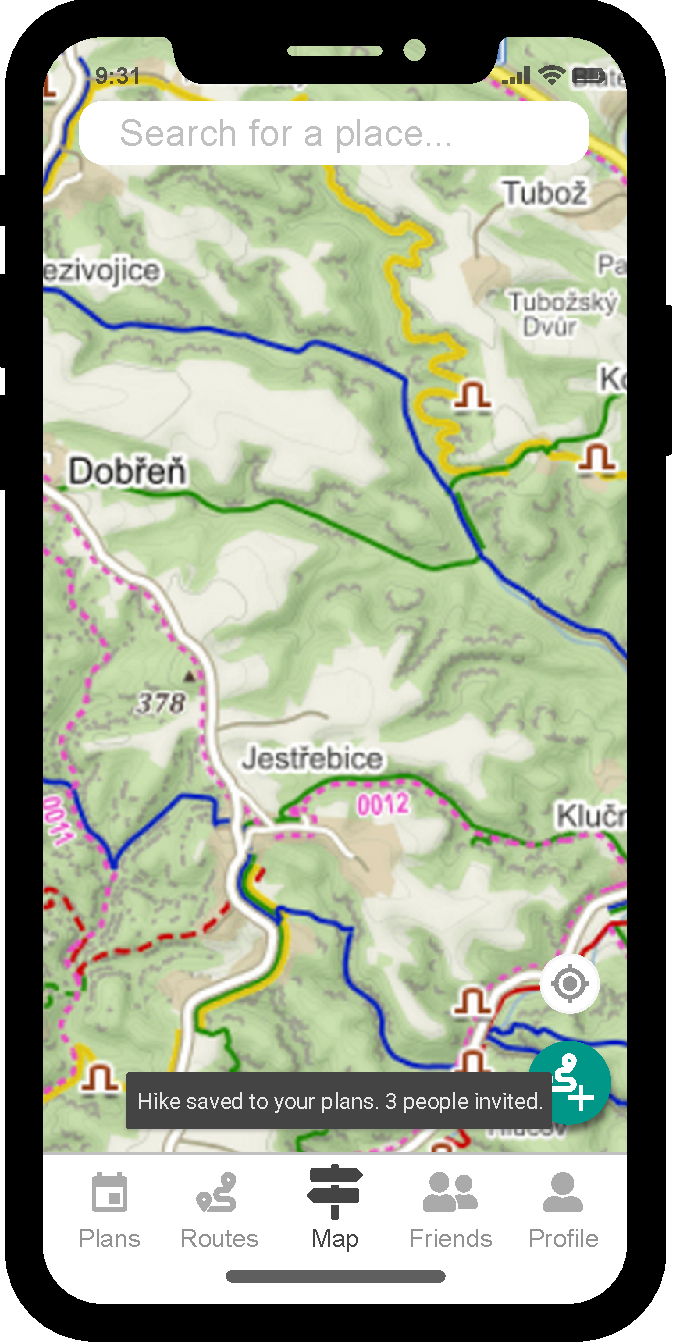
\includegraphics[width=0.4\textwidth]{Images/appScreens/map-plan9.pdf}}\hfill
    \caption{Overview of the hike. After pressing the `Finish' button, we are back to the `Map' screen.}
    \label{fig:plan-end}
\end{figure}

\section{Plans tab}
The `Plans' tab is divided into three sections -- `All plans', `My plans' and `History'.
The default `All plans' section~(fig.\ref{fig:plan-all-plans}) is a filterable feed of the users' and their friends' upcoming plans (US~\ref{US:friends-join-hikes}).
This is also where the user's invitations to friends' hikes are displayed; these can be either dismissed or accepted (US~\ref{US:friends-invite-accept}}, \ref{US:friends-invite-refuse}).

A collapsed hike card contains basic information, the route on a map (represented by the picture placeholder) such as who hosts it, when it is happening and how long it will take, whether it is joinable and how difficult it would be for the user.

When tapping on the card, the card expands to show more of the hike's details: 
who is coming, how long it is currently planned to be plus how much longer it will take if the user joins, and all of its information recalculated to the user's fitness.

If the hike is joinable, there is an `Ask to join' button (US~\ref{US:friends-join-hikes}); if not, the user can only go back.

Again, there are the options to save (US~\ref{US:map-saved}) or share the route (US~\ref{US:map-share-route}).

\begin{figure}[h!]
    \centering
    \tmpframe{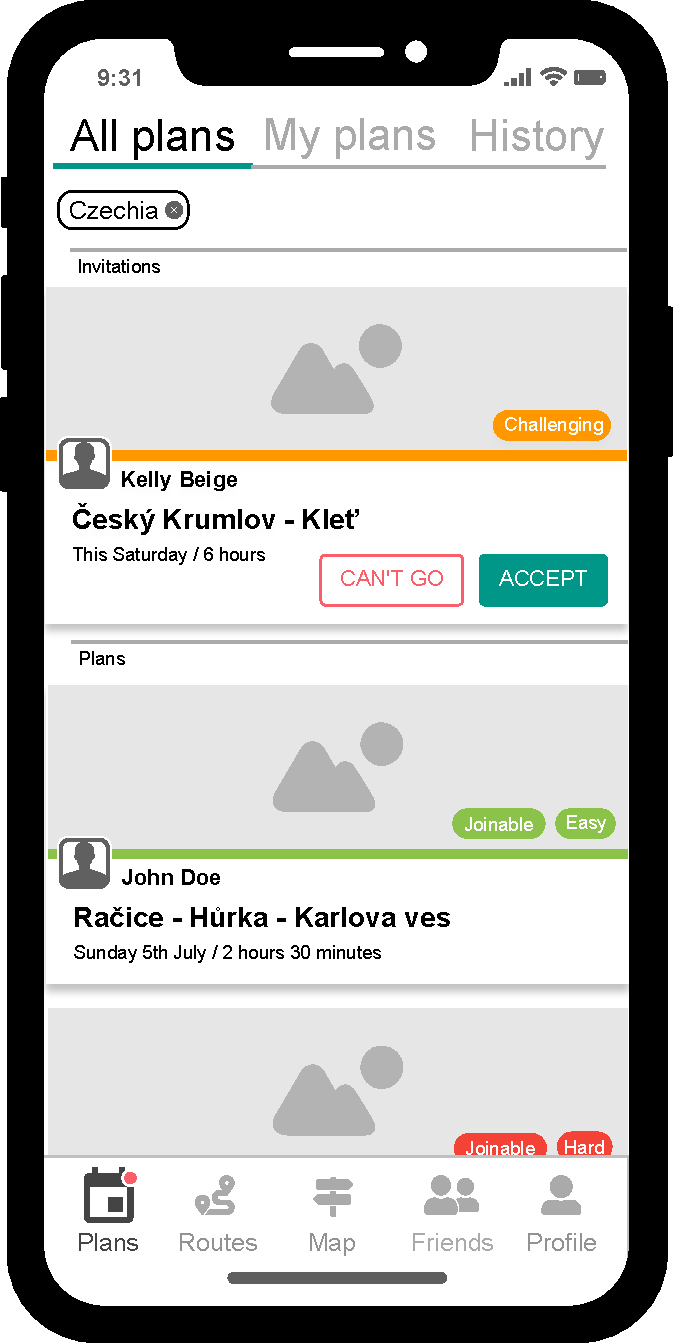
\includegraphics[width=0.4\textwidth]{Images/appScreens/plans-all-plans.pdf}}\hfill
    \tmpframe{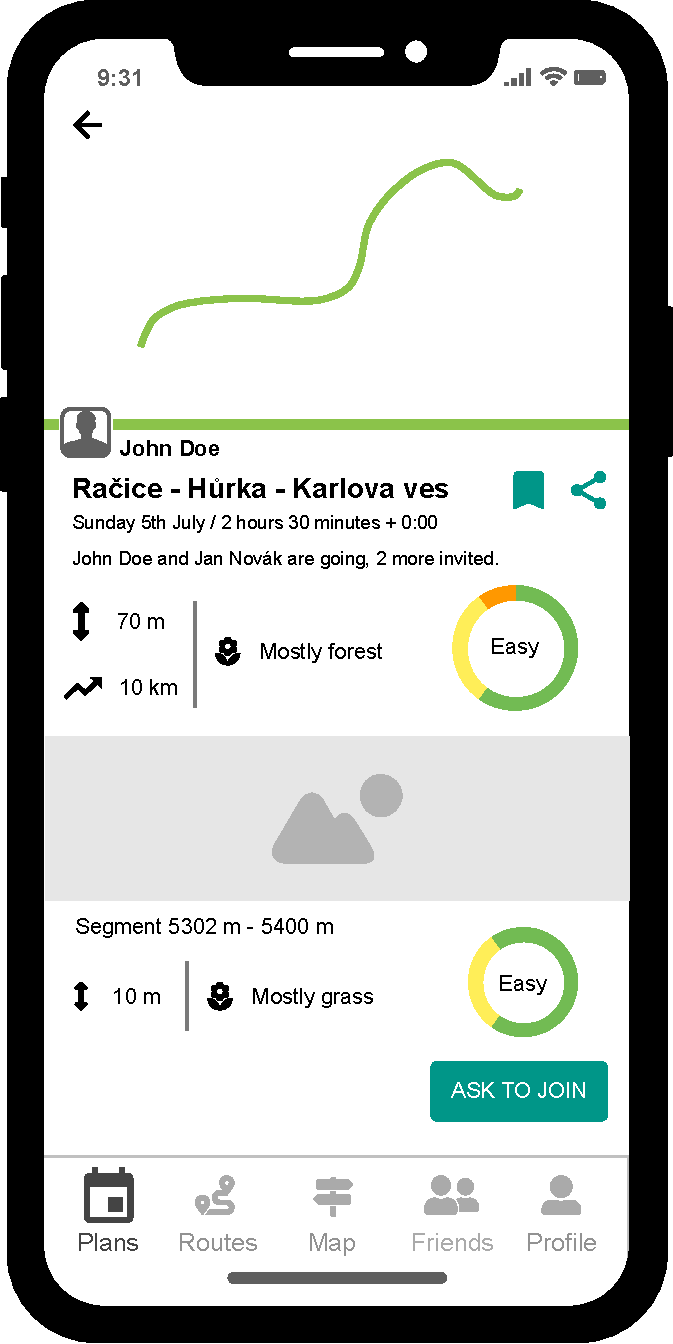
\includegraphics[width=0.4\textwidth]{Images/appScreens/plans-all-plans-joinable-detail.pdf}}\hfill
    \caption{All plans feed. Detail of a joinable hike.}
    \label{fig:plan-all-plans}
\end{figure}

The `My plans' section~(fig.\ref{fig:plan-my-plans}) contains the hikes that the user has planned or joined.
The detail of a hike planned by the user is different, compared to looking at hikes planned by other people,
since there have to be options to administer the hike.
Requests to join are shown in this detail; by tapping at the `People' section the user can manage the people connected to the hike, as well as allow or disallow people to join the hike (US~\ref{US:friends-join-hikes}).
The route can be cancelled by the red trash icon, and the user can also let others know that they can't go (US~\ref{US:friends-cancel-hike}).
If the user is the host of the hike, they have to appoint a new host from the people who have accepted the invitation.

The `Start' button will become active on the day of the hike.
When it is pressed, the route will be activated on the phones of all the attendants, allowing to switch to navigation mode (US~\ref{US:friends-hike-active}).

Tapping on the `Route' section will show the route's details, just like in fig.\ref{fig:plan-pick-route}.

\begin{figure}[h!]
    \centering
    \tmpframe{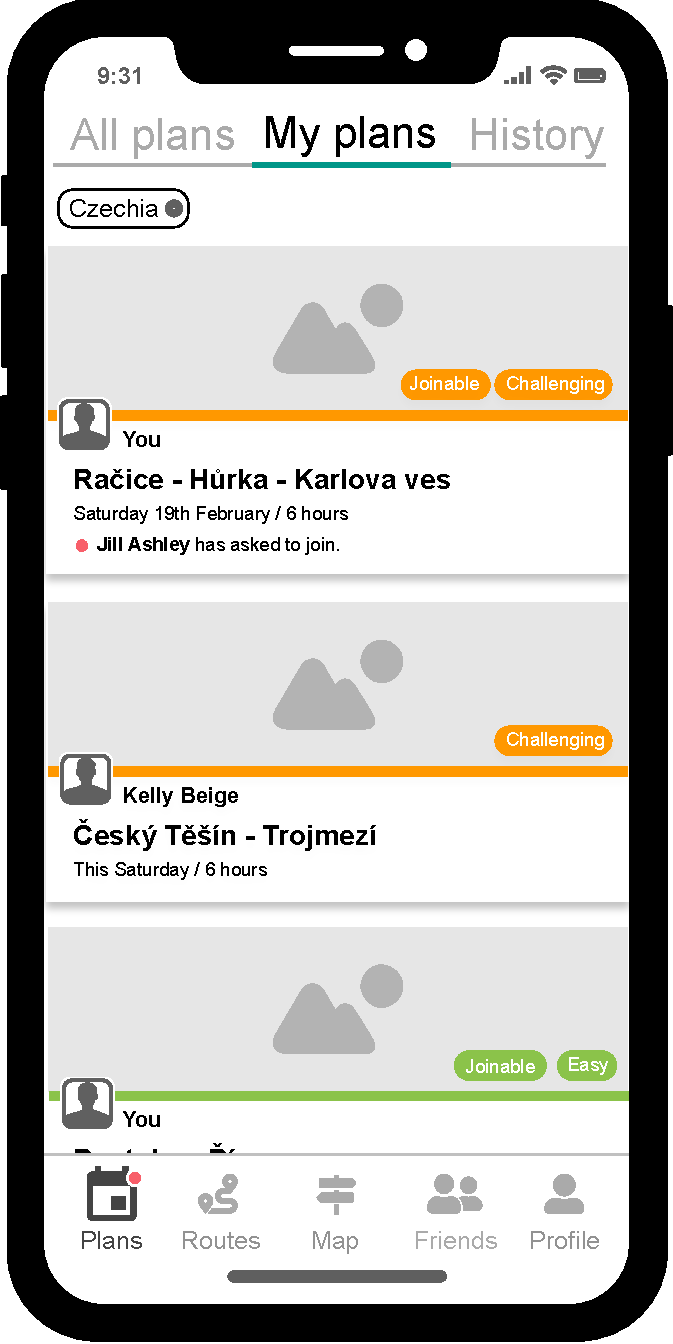
\includegraphics[width=0.3\textwidth]{Images/appScreens/plans-my-plans.pdf}}\hfill
    \tmpframe{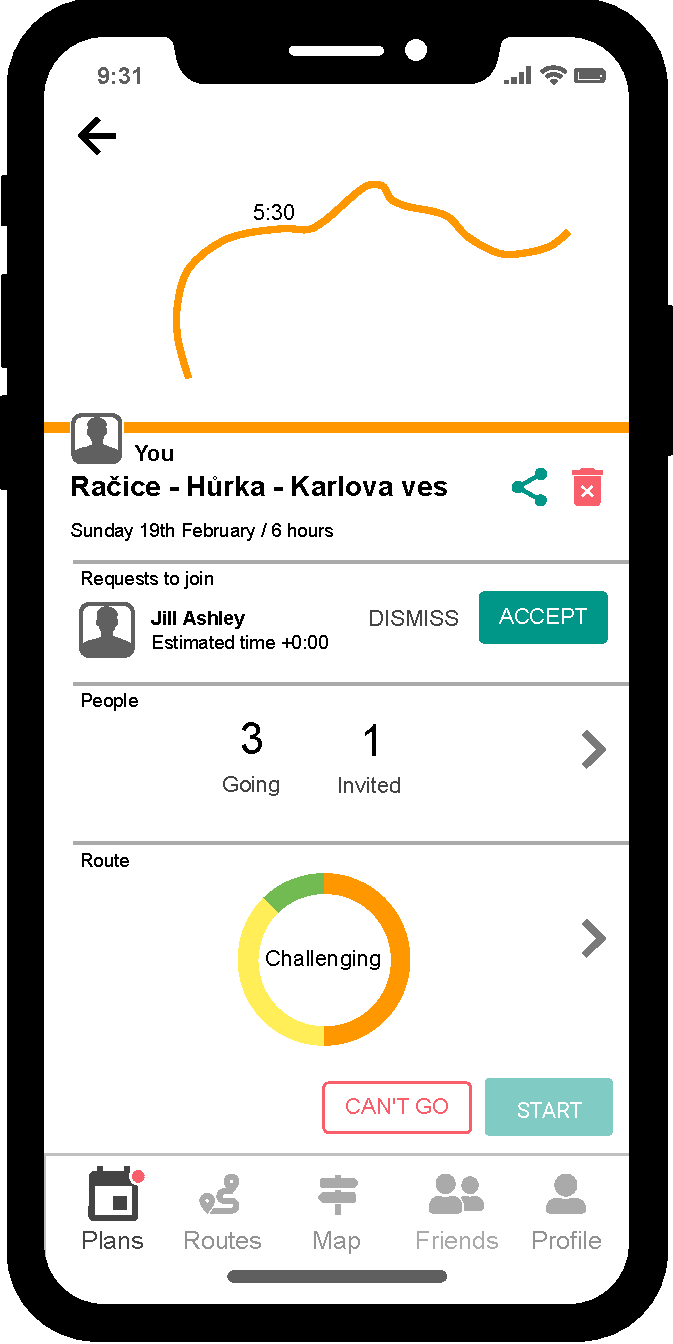
\includegraphics[width=0.3\textwidth]{Images/appScreens/plans-my-plans-detail.pdf}}\hfill
    \tmpframe{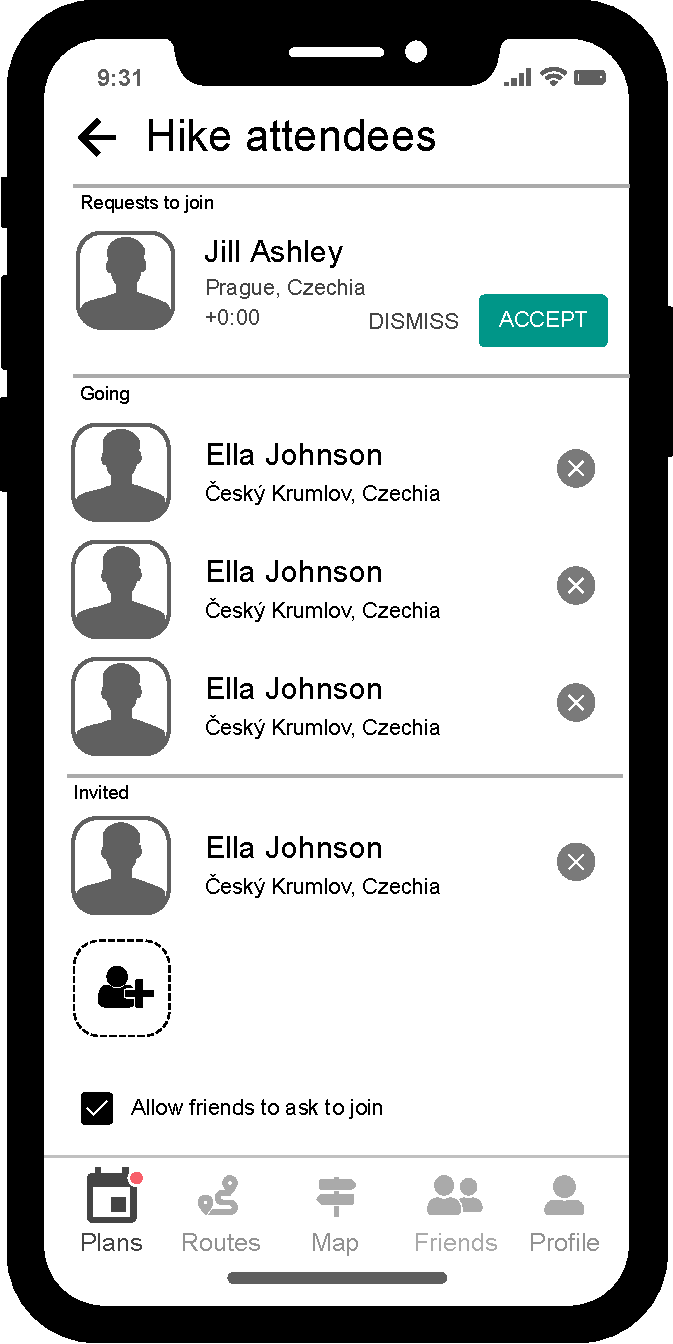
\includegraphics[width=0.3\textwidth]{Images/appScreens/plans-my-plans-detail-people.pdf}}\hfill
    \caption{My plans. Detail of a hike planned by the user, and a view of the invited and going people.}
    \label{fig:plan-my-plans}
\end{figure}

The `history' section~(fig.\ref{fig:plan-history}) of the `Plans' tab is the same as the `My plans' section, except all the hikes are in the past (US~\ref{US:map-history}).
Each hikes' map contains the planned route, and the real route in case the user didn't precisely follow the plan.
This hike can be repeated by pressing the `Plan a hike' button and choosing whether to use the originally planned or the actually taken route.
Then the user is again taken to the planning UI.

\begin{figure}[h!]
    \centering
    \tmpframe{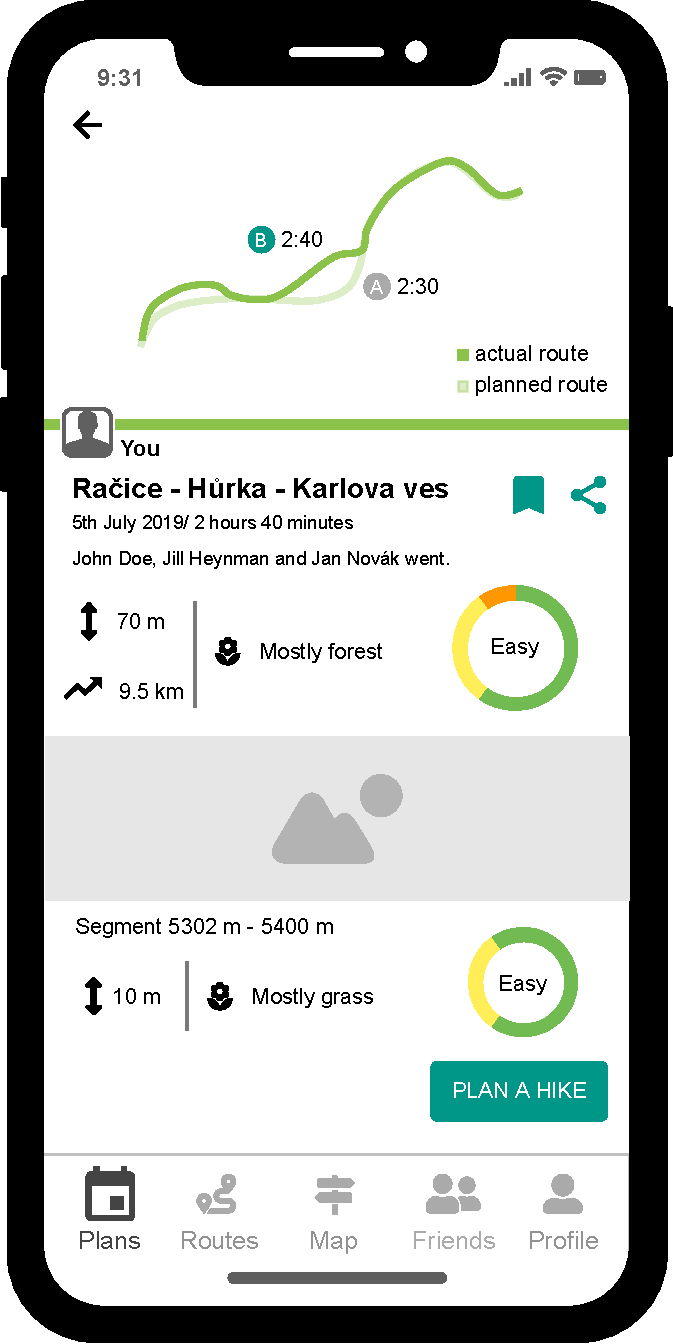
\includegraphics[width=0.4\textwidth]{Images/appScreens/plans-history-detail.pdf}}\hfill
    \caption{Detail of a historic hike.}
    \label{fig:plan-history}
\end{figure}

\section{Routes tab}
The `Routes' tab~(fig.\ref{fig:routes}) contains a filterable list of saved routes (US~\ref{US:map-saved}).
The only difference between a hike card and a route card is the fact that routes are not planned, so they don't include a host, people who are going, or the date they are planned for.

\begin{figure}[h!]
    \centering
    \tmpframe{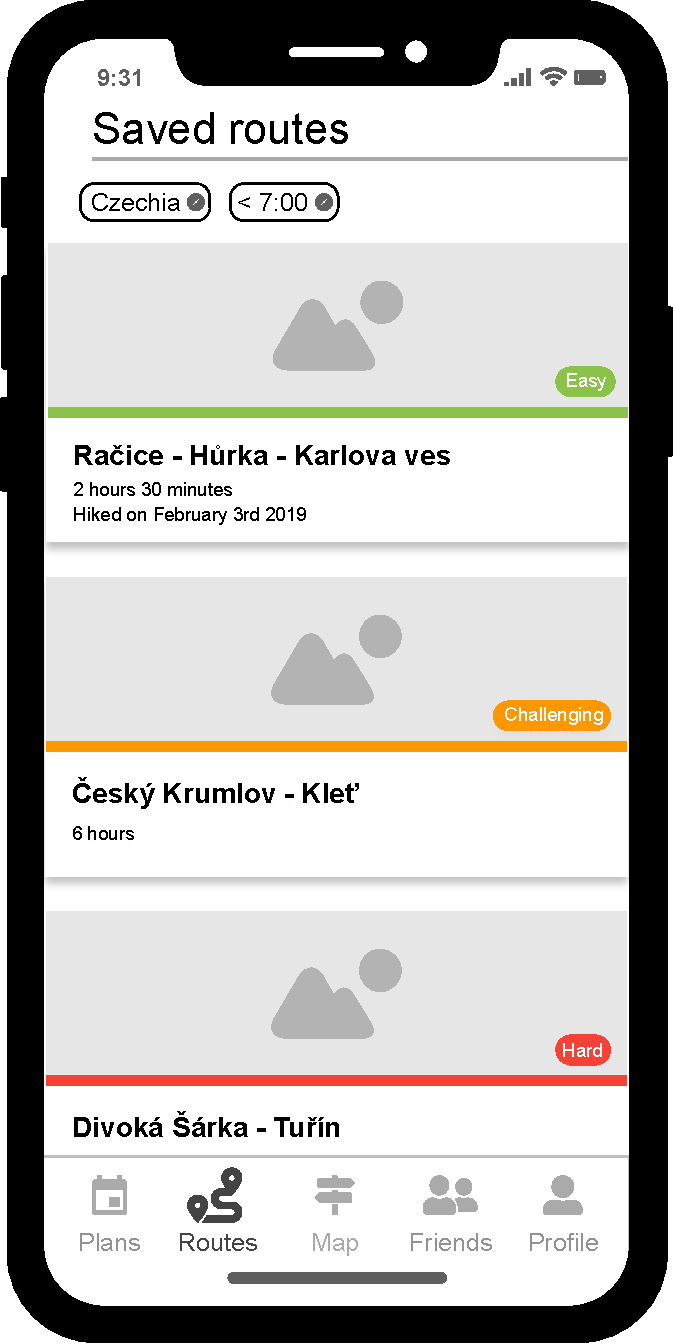
\includegraphics[width=0.4\textwidth]{Images/appScreens/routes.pdf}}\hfill
    \tmpframe{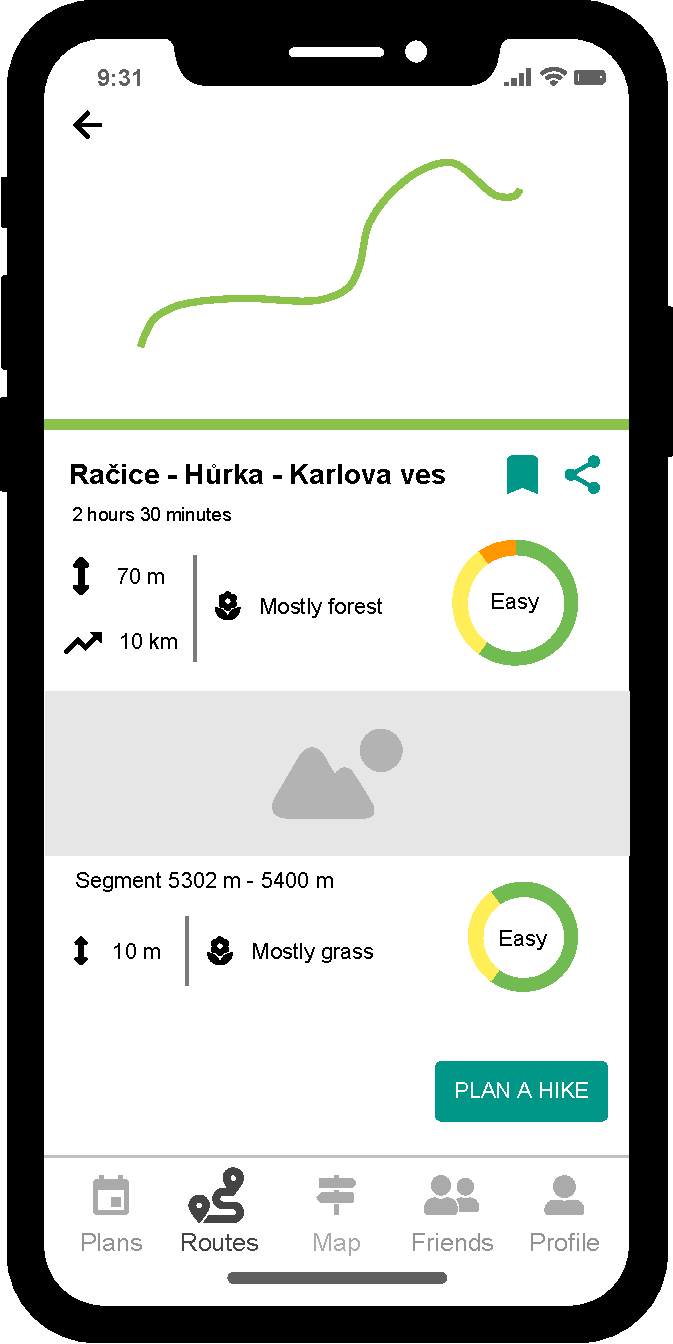
\includegraphics[width=0.4\textwidth]{Images/appScreens/routes-detail.pdf}}\hfill
    \caption{Routes tab. Detail of a route.}
    \label{fig:routes}
\end{figure}

\section{Friends tab}
Finally, the last tab is the `Friends' tab.
It contains a view of all the user's friends, as well as any pending friendship requests (US~\ref{US:friends-accept}, \ref{US:friends-dismiss}).
The detail of a user's profile is similar to the user who is signed in, but contains only basic information.
The profile is shareable (US~\ref{US:friends-share}), and the friend can also be removed from the user's friends list (US~\ref{US:friends-remove}).
This is confirmed by a confirmation dialogue, warning the user about the fact that they will be removed from one another's plans.

Using the add button, the user can also add new friends using a link or social media (fig.\ref{fig:friends}; US~\ref{US:friends-add}).

\begin{figure}[h!]
    \centering
    \tmpframe{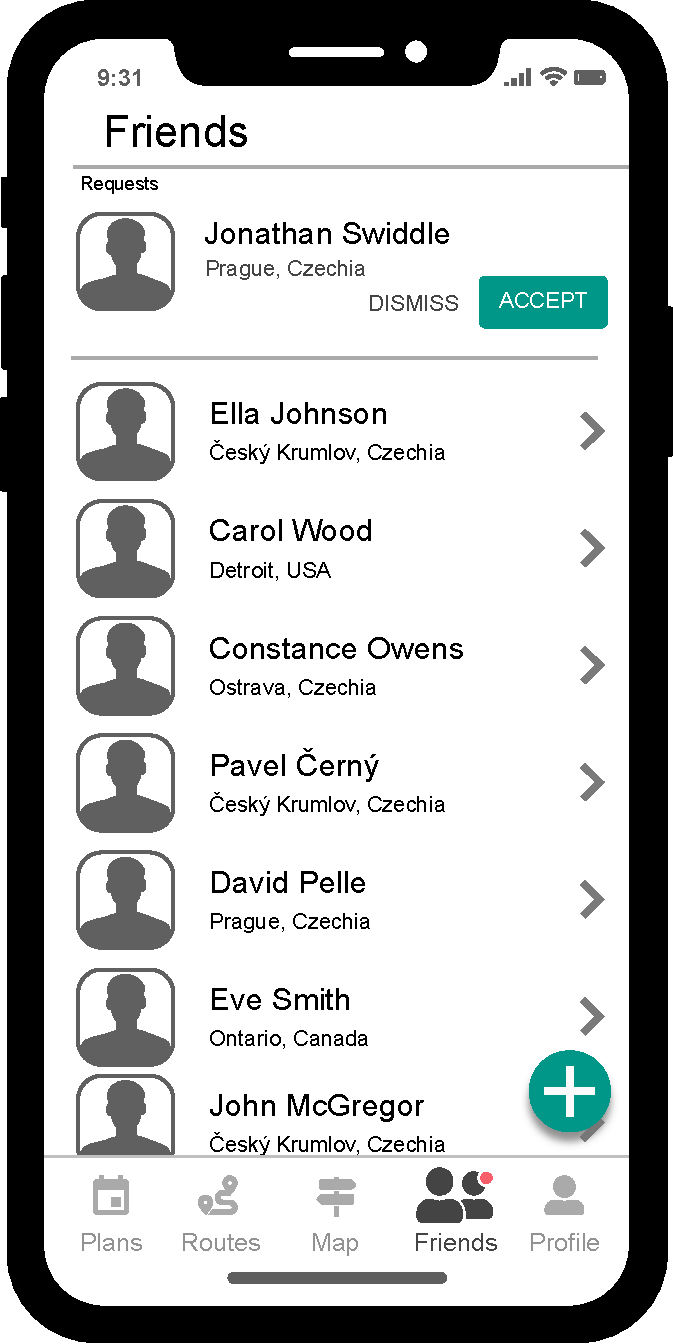
\includegraphics[width=0.3\textwidth]{Images/appScreens/friends.pdf}}\hfill
    \tmpframe{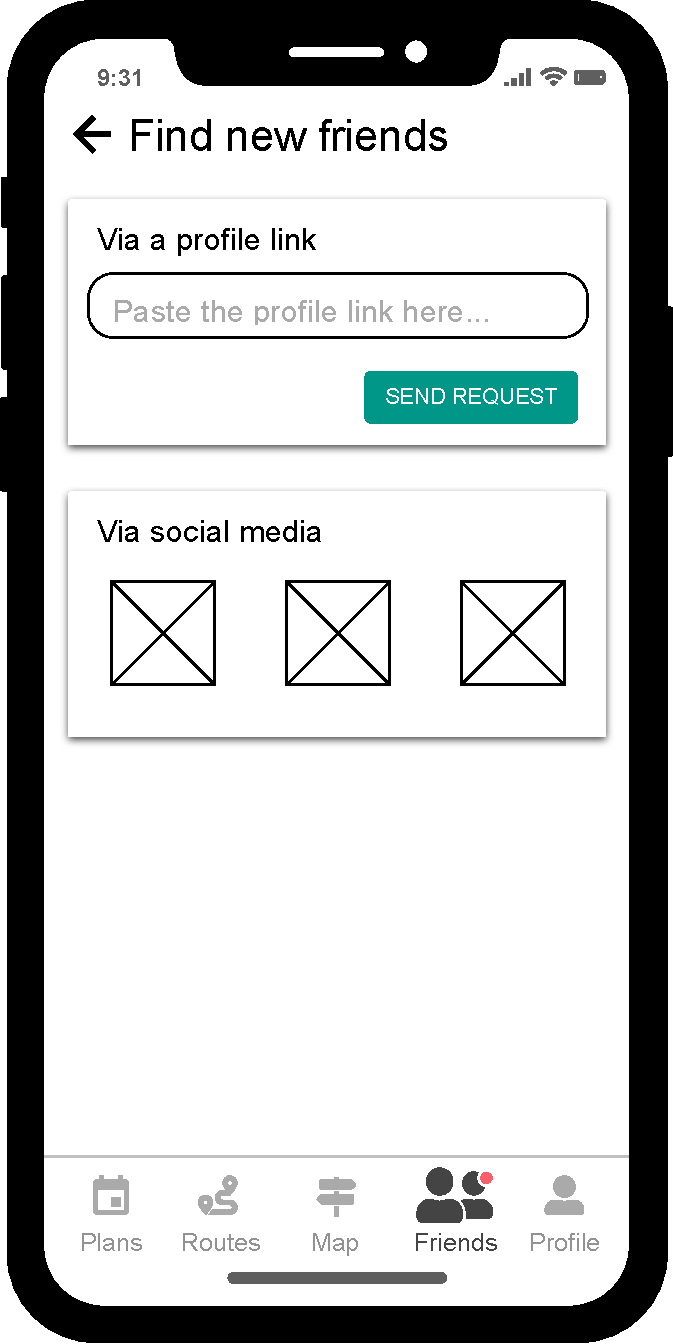
\includegraphics[width=0.3\textwidth]{Images/appScreens/friends-find.pdf}}\hfill
    \tmpframe{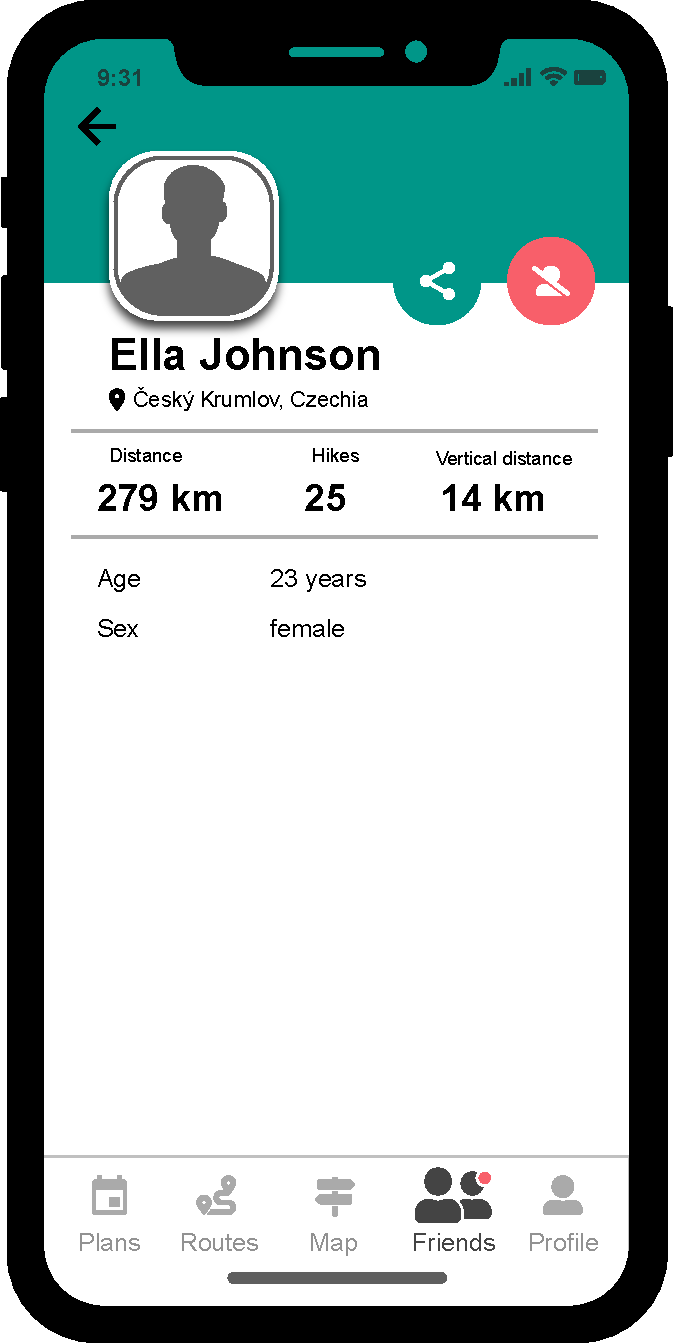
\includegraphics[width=0.3\textwidth]{Images/appScreens/friends-detail.pdf}}
    \caption{Friends tab, finding new friends and the user profile of a friend.}
    \label{fig:friends}
\end{figure}

\section{Navigation mode}
The application allows a user to navigate a planned route using a map and written directions (fig.\ref{fig:navigation}; US~\ref{US:map-hike}).
Once a hike is started, the view is switched to the `Map' tab.
The route is visualized on the map in colours of respective hiking trails and the user's position is highlighted.
There's also an overview of the difficulty of the current part of the route, and the user is notified if they are lagging behind the plan.
If the user wants to see something else than the navigation mode, they can use the close button on the top right, or just switch between tabs.
The navigation mode stays alive and accessible through a permanent notification.

\begin{figure}[h!]
    \centering
    \tmpframe{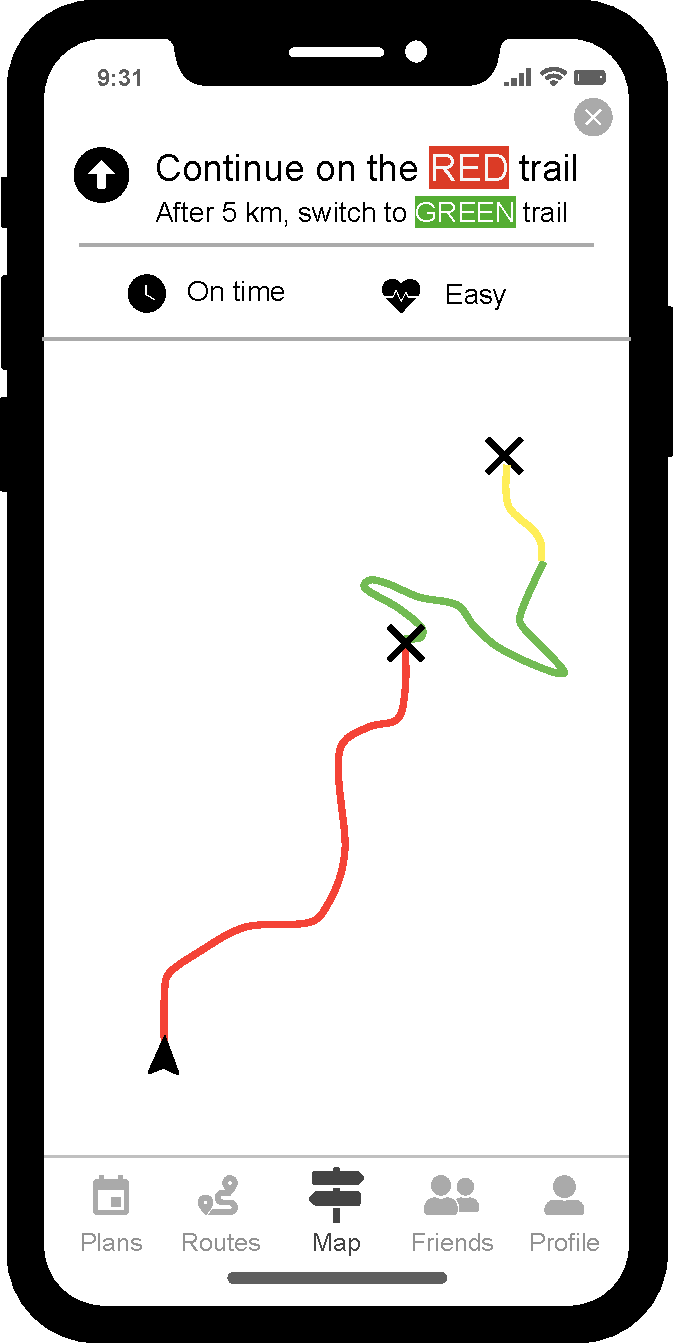
\includegraphics[width=0.4\textwidth]{Images/appScreens/navigation.pdf}}
    \label{fig:navigation}
\end{figure}

\section{Notifications}
Notifications are communicated to the user via icon badges on the bottom tab bar.

Notifications are primarily sent to the system and are displayed on the notification bar.
